\documentclass[twoside]{article}
\usepackage{lmodern}
\usepackage{textcomp}
\usepackage[T1]{fontenc}
\usepackage[utf8x]{inputenc}
%\usepackage{ltexpprt} 
%\usepackage{balance}
\usepackage[numbers,sort&compress,comma]{natbib}
\usepackage[bookmarks=true,pdfstartview={FitH},pdfauthor={Matteo Riondato
and Fabio Vandin},pdftitle={Finding the True Frequent Itemsets},pdfsubject={Frequent Itemsets Mining}]{hyperref}
\usepackage[ruled,linesnumbered]{algorithm2e} % must load after natbib
\usepackage{fullpage}
%\usepackage{amsfonts}
\usepackage{amsmath}
\usepackage{amssymb}
\usepackage{dsfont}
\usepackage{amsthm}
\usepackage{mathtools}
\usepackage{graphicx}
%\usepackage{subfig}
\usepackage{multirow}
%\usepackage{bigstrut}
%\usepackage{url}
\usepackage{mdwlist}
\usepackage{booktabs}
%\usepackage{savesym}
%\savesymbol{algorithm}
%\savesymbol{endalgorithm}
\usepackage{datetime}
%\usepackage{times}
%\usepackage{mathptm}
%\DeclareSymbolFont{largesymbols}{OMX}{psycm}{m}{n}
%\usepackage[usenames,dvipsnames,svgnames,table]{xcolor}


%\renewcommand\bibnumfmt[1]{[#1]} 
%\renewcommand{\bibsection}{\section{\refname}}

%\def\newblock{\hskip .11em plus .33em minus .07em}
%\DeclareCaptionType{copyrightbox}

%\def\qed{}
\def\Sam{{\cal S}}
\def\Ds{{\cal D}}
\def\Itm{{\cal I}}
\def\FI{\mathsf{FI}}
\def\TFI{\mathsf{TFI}}
\def\VC{\mathsf{VC}}
\def\EVC{\mathsf{EVC}}
\def\prob{\pi}
\def\tfreq{t_\prob}
\def\range{\mathcal{R}}
\def\eb{\mathsf{eb}}
%\def\b{\mathsf{b}}
\def\ALG{{\sf TFI-VC}}
\def\ALGHOLDOUT{{\sf TFI-H}}

\newtheorem{corollary}{Corollary}
%\newtheorem{conj}{Conjecture}
\newtheorem{lemma}{Lemma}
%\newtheorem{claim}{Claim}
\newtheorem{fact}{Fact}
\newtheorem{theorem}{Theorem}

\theoremstyle{definition}
\newtheorem{definition}{Definition}

%\newcommand{\fabio}[1]{\textcolor{blue}{#1}}
%\usepackage[normalem]{ulem}


\begin{document}
\title{Finding the True Frequent Itemsets\thanks{Work supported in part by NSF
grant IIS-1247581.
\ifarxiv
 This is an extended version of the work that appeared
as~\citep{RiondatoV14}.
\fi
}
}
\author{Matteo Riondato
\ifarxiv
\thanks{Department of Computer Science, Brown University, Providence, RI, USA.
\url{matteo@cs.brown.edu}. Contact author.}
\else
\thanks{Brown University, Providence, RI, USA}
\fi
\and Fabio Vandin
\ifarxiv
\thanks{Department of Computer Science, Brown University, Providence, RI, USA
and Department of Mathematics and Computer Science, University of Southern
Denmark, Odense, Denmark. \url{vandinfa@imada.sdu.dk}.}
\else
\textsuperscript{$\dagger$,}\thanks{University of Southern Denmark, Odense, Denmark}
\fi
}

\date{\today}

\maketitle

\begin{abstract} 
   Frequent Itemsets (FIs) mining is a fundamental primitive in knowledge
   discovery. It requires to identify all itemsets appearing in at least a
   fraction $\theta$ of a transactional dataset $\Ds$. Often though, the
   ultimate goal of mining $\Ds$ is not an analysis of the dataset \emph{per
   se}, but the understanding of the underlying process that generated $\Ds$.
   Specifically, in many applications $\Ds$ is a collection of samples obtained
   from an unknown probability distribution $\prob$ on transactions, and by
   extracting the FIs in $\Ds$ one attempts to infer itemsets that are
   frequently (i.e., with probability at least $\theta$) generated by $\prob$,
   which we call the True Frequent Itemsets (TFIs). Due to the inherently
   stochastic nature of the generative process, the set of FIs is only a rough
   approximation of the set of TFIs, as it often contains a huge number of
   \emph{false positives}, i.e., spurious itemsets that are not among the TFIs.
   In this work we design and analyze an algorithm to identify a threshold
   $\hat{\theta}$ such that the collection of itemsets with frequency at least
   $\hat{\theta}$ in $\Ds$ contains only TFIs with probability at least
   $1-\delta$, for some user-specified $\delta$. Our method uses results from
   statistical learning theory involving the (empirical) VC-dimension of the
   problem at hand. This allows us to identify almost all the TFIs without
   any false positive.  We also experimentally compare our method with
   the direct mining of $\Ds$ at frequency $\theta$ and with techniques based on
   widely-used standard bounds (i.e., the Chernoff bounds) of the binomial
   distribution, and show that our algorithm outperforms these methods and
   achieves even better results than what is guaranteed by the theoretical
   analysis.
 \end{abstract}

%{\bf Categories and Subject Descriptors:} H.2.8 [Database Management]: Database Applications -- \emph{Data Mining}

{\bf Keywords:} Frequent itemsets, VC-dimension, False positives,
Distribution-free methods, Frequency threshold identification, Pattern mining,
Significant patterns.


\section{Introduction}\label{sec:intro}

The extraction of association rules is one of the fundamental primitives in data
mining and knowledge discovery from large databases~\citep{AgrawalIS93}.  In its
most general definition, the problem can be reduced to identifying frequent sets
of items, or \emph{Frequent Itemsets} (FIs), appearing in at least a fraction
$\theta$ of all transactions in a dataset, where $\theta$ is provided in input
by the user. Frequent itemsets and association rules are not only of interest
for classic data mining applications (e.g., market basket analysis), but are
also useful for further data analysis and mining task, including clustering,
classification, and indexing~\citep{han2006data,HanCXY07}.

In most applications, the collection of FIs is not interesting \emph{per se}.
Instead, the mining results are used to infer properties of the \emph{underlying
process} that generated the dataset. Consider for example the following
scenario: a team of researchers would like to identify frequent associations
(i.e., itemsets) between preferences among Facebook users. To this end, they set
up an online survey which is filled out by a \emph{small fraction} of Facebook
users (some users may even take the survey multiple times). Using this
information, the researchers want to infer the associations (itemsets) that are
frequent for the \emph{entire} Facebook population. In fact, the whole Facebook
population and the online survey define the underlying \emph{process} that
generated the dataset \emph{observed} by the researchers. In this work we are
interested in answering the following question: how can we use the latter (the
observed dataset) to identify itemsets that are frequent in the former (the
whole population)? This is a very natural question, as is the underlying
assumption that the observed dataset is \emph{representative} of the generating
process. For example, in market basket analysis, the observed purchases of
customers are used to infer the future purchase habits of all customers while
assuming that the purchase behavior that generated the dataset is representative
of the one that will be followed in the future.

A natural and general model to describe these concepts is to assume that the
transactions in the dataset $\Ds$ are \emph{independent identically distributed}
(i.i.d.) samples from an \emph{unknown} probability distribution $\prob$ defined
on all possible transactions built on a set of items. Since $\prob$ is fixed,
each itemset $A$ has a fixed (unknown) \emph{probability} $\tfreq(A)$ to appear
in a transaction sampled from $\prob$. We call $\tfreq(A)$ the \emph{true
frequency} of $A$ (w.r.t.~$\prob$). The true frequency corresponds to the
fraction of transactions that would contain the itemset $A$ among an
hypothetical infinite set of transactions. The real goal of the mining process
is then to identify itemsets that have true frequency $\tfreq$ at least
$\theta$, i.e., the \emph{True Frequent Itemsets} (TFIs). In the market basket
analysis example, $\Ds$ contains the observed purchases of customers, the
\emph{unknown} distribution $\prob$ describes the purchase behavior of the
customers as a whole, and we want to analyze $\Ds$ to find the itemsets that
have probability (i.e., true frequency) at least $\theta$ to be bought by a
customer. Note that we made no assumption on $\prob$, except from the fact that
the transactions in the dataset are i.i.d.~samples from $\prob$. This is in
contrast to other settings that assume that the generative distribution $\prob$
is such that items appear in transactions generated by $\prob$ totally or
partially independently from each
other~\citep{SilversteinBM98,MegiddoS98,DuMouchelP01,GionisMMT07,Hamalainen10,KirschMAPUV12}.

Since $\Ds$ represents only a \emph{finite} sample from $\prob$, the set $F$ of frequent itemsets
of $\Ds$ w.r.t.~$\theta$ only provides an \emph{approximation} of the True Frequent Itemsets:
due to the stochastic nature of the generative process, the set $F$ may contain
a number of \emph{false positives}, i.e., itemsets that appear among the
frequent itemsets of $\Ds$ but whose \emph{true} frequency is smaller than
$\theta$.  At the same time, some itemsets with true frequency greater than
$\theta$ may have a frequency in $\Ds$ that is \emph{smaller} than $\theta$
(\emph{false negatives}), and therefore not be in $F$. This implies that one can
not aim at identifying \emph{all and only} the itemsets having true frequency at
least $\theta$. Even worse, from the data analyst's point of view, there is
\emph{no guarantee or bound on the number of false positives} reported in $F$.
Consider the following scenario as an example. Let $A$ and $B$ be two (disjoint)
sets of pairs of items. The set $A$ contains 1,000 disjoint pairs, while $B$
contains 10,000 disjoint pairs. Let $\prob$ be such that, for any pair
$(a,a')\in A$, we have $\tfreq((a,a'))=0.1$, and for any pair $(b,b')\in B$, we
have $\tfreq((b,b'))=0.09$. Let $\Ds$ be a dataset of 10,000 transactions
sampled from $\prob$. We are interested in finding pairs of items that have true
frequency at least $\theta=0.095$. If we extract the pairs of items with
frequency at least $\theta$ in $\Ds$, it is easy to see that in expectation 50
of the 1,000 pairs from $A$ will have frequency in $\Ds$ \emph{below} $0.095$,
and in expectation 400 pairs from $B$ will have frequency in $\Ds$ \emph{above}
$0.095$.  Therefore, the set of pairs that have frequency at least $\theta$ in
$\Ds$ does \emph{not} contain some of the pairs that have true frequency at
least $\theta$ (false negatives), but includes a huge number of pairs that have
true frequency smaller than $\theta$ (false positives).

In general, one would like to avoid false positives and at the same time find as
many TFIs as possible. These are somewhat contrasting goals, and care must be
taken to strike a good balance between them.  A na\"ive but \emph{overly
conservative} method to avoid false positives involves the use of \emph{Chernoff
and union bounds}~\citep{MitzenmacherU05}.  Let $A$ be an itemset in $\Ds$, and
$f_\Ds(A)$ be its frequency in the dataset, i.e., the fraction of transactions
of $\Ds$ that contain $A$. The quantity $|\Ds|f_\Ds(A)$ is a random variable
with Binomial distribution $\mathcal{B}(|\Ds|,\tfreq(A))$. It is possible to use
standard methods like the Chernoff and the union bounds to bound the deviation
of the frequencies in the dataset of \emph{all} itemsets from their
expectations. These tools can be used to compute a value $\hat\theta$ such that
the probability that a non-true frequent itemset $B$ has frequency greater or
equal to $\hat\theta$ is at most $1-\delta$, for some $\delta\in(0,1)$. This
method has the following serious drawback: in order to achieve such guarantee,
it is \emph{necessary} to bound the deviation of the frequencies of \emph{all
itemsets possibly appearing in the dataset}~\citep{KirschMAPUV12}. This means
that, if the transactions are built on a set of $n$ items, the union bound must
be taken over all $2^n-1$ potential itemsets, even if some or most of them may
appear with very low frequency or not at all in samples from $\prob$. As a
consequence, the chosen value of $\hat\theta$ is extremely \emph{conservative},
despite being sufficient to avoid the inclusion of false positives in the mining
results. The collection of itemsets with frequency at least $\hat\theta$ in
$\Ds$, although consisting (probabilistically) only of TFIs, only contains a
\emph{very small} portion of them, due to the overly conservative choice of
$\hat\theta$. (The results of our experimental evaluation in
Sect.~\ref{sec:experiments} clearly show the limitations of this method.) More
refined algorithms are therefore needed to achieve the correct balance between
the contrasting goals of avoiding false positives and finding as many TFIs as
possible.

\subsection{Our contributions.}
The contributions of this work are the following:
\begin{itemize*}
	\item We formally define the problem of mining the \emph{True Frequent
	Itemsets} w.r.t.~a minimum threshold $\theta$, and we develop and analyze an
	algorithm to \emph{identify a value $\hat{\theta}$ such that, with
	probability at least $1-\delta$, all itemsets with frequency at least
	$\hat{\theta}$ in the dataset have true frequency at least $\theta$}. Our
	method is completely \emph{distribution-free}, i.e., it does not make
	\emph{any} assumption about the unknown generative distribution $\prob$. By
	contrast, existing methods to assess the significance of frequent patterns
	after their extraction require a well specified, limited generative model to
	characterize the significance of a pattern. Our method also allows to
	include additional prior information about the distribution $\prob$, when
	available, to obtain even higher accuracy.
	\item We analyze our algorithm using results from \emph{statistical learning
	theory} and \emph{optimization}. We define a range set associated to a
	collection of itemsets and give an upper bound to its (empirical)
	VC-dimension and a procedure to compute this bound, showing an interesting
	connection with the Set-Union Knapsack Problem
	(SUKP)~\citep{GoldschmidtNY94}. To the best of our knowledge, ours is the
	first work to apply these techniques to the field of TFIs, and in general
	the first application of the sample complexity bound based on
	\emph{empirical} VC-dimension to the field of data mining.
	\item We implemented our algorithm and assessed its performances on
	simulated datasets with properties (number of items, itemsets frequency
	distribution, etc.) similar to real datasets. We computed the fraction of
	TFIs contained in the set of frequent itemsets in $\Ds$ w.r.t.~$\hat\theta$,
	and the number of false positives, if any. The results show that the
	algorithm is even \emph{more accurate} than the theory guarantees, since
	\emph{no false positive} is reported in any of the many experiments we
	performed, and moreover allows the \emph{extraction of almost all TFIs}. We
	also compared the set of itemsets computed by our method to those obtained
	with the ``Chernoff and union bounds'' method presented in the introduction,
	and found that our algorithm \emph{vastly outperforms} it.
\end{itemize*}

\paragraph*{Outline.}
\fabio{[TO BE UPDATED.]}
In Sect.~\ref{sec:prevwork} we review relevant previous contributions.
Sections~\ref{sec:prelims} and~\ref{sec:range} contain preliminaries to formally
define the problem and key concepts that we will use throughout the work. Our
proposed algorithm is described and analyzed in Sect.~\ref{sec:main}. We present
the methodology and results of our experimental evaluation in
Sect.~\ref{sec:experiments}.  Conclusions and future directions can be found in
Sect.~\ref{sec:concl}.

%This is an example of a statistical test, in which the probability, or $p$-value,
%that a measure, or \emph{statistic} (in the example, the frequency of $\{a,b\}$)
%is at least as extreme as the value observed in real data is computed under a
%\emph{null hypothesis} that captures the properties of spurious discoveries (in
%the example, the independence of items). When the $p$-value is small enough, the
%itemset is flagged as significant, otherwise the itemset is discarded as a
%spurious discovery. A number of different
%procedures~\citep{SilversteinBM98,MegiddoS98,DuMouchelP01,GionisMMT07,Hamalainen10,KirschMAPUV12}
%have been proposed
%in recent years to control the number of spurious discoveries that are reported
%\emph{after} the frequent itemsets are identified. These procedures take into
%account the fact that a transactional dataset contains a number of patterns, and
%the assessment of their significance therefore is a \emph{multiple
%hypothesis testing} problem.
%
%
%For example, consider
%the transactions given by items that are bought together on Amazon; after
%observing a certain number of transactions, one is interested in inferring
%association between items that are valid for the distribution over \emph{all} possible
%purchases, not only for the current, observed set $\Ds$ of purchases that
%represents only a partial observation obtained from the distribution that
%includes also purchases that have not been recorded in the dataset, or that will
%materialize only in the future.
%
%The itemsets that are not frequent in $p$ but are frequent in $\Ds$ are false
%discoveries, and are not going to be filtered by the statistical tests described
%above, since such tests \emph{assume} that the itemsets that are frequent in
%$\Ds$, whose significance they assess, represent the frequent itemsets in $p$ as
%well. In fact, these tests define itemsets as spurious by considering properties
%of the itemsets other than its frequency. In the example above, the
%co-occurrence of $\{a,b\}$ is likely not due to random chance; however, the
%probability that $\{a,b\}$ appears with frequency $3\%$  in $\Ds$ while its
%frequency in $p$ is $1\%$ is $0.08$, therefore if $\theta=2\%$ then $\{a,b\}$
%likely is a false discovery. As noted by~\citet{LiuZW11}, the phase of
%assessment of the significance of the frequent itemsets cannot replace the role
%played by the minimum support threshold $\theta$, that is to reflect the level
%of domain significance, and is to be used in concert with statistical
%significance to filter uninteresting patterns that arise from different sources.
%Therefore being able to rigorously identify frequent patterns in $p$ is crucial
%in order to obtain high quality patterns.
%
%In this paper we address the problem of identifying itemsets that appear with
%probability at least $\theta$ in $p$, that we call \emph{True Frequent Itemsets}
%(RFI), while providing rigorous probabilistic guarantees on the number of false
%discoveries, without making any assumption on the particular generative model of
%the transactions. This makes our method completely \emph{distribution free}. In
%particular, we focus on returning a set of RFI with bounded Family-Wise Error
%Rate (FWER), that is the probability that one or more false discovery is
%reported among the RFI. A recently proposed alternative to  bound the FWER is to
%bound the False Discovery Rate (FDR), that in our case correspond to the
%proportion of false discoveries among the RFI. The use of the FDR allows to
%produce in output a larger number of patterns, since a small proportion of false
%discoveries are tolerated in the output; however, in data mining the number of
%patterns produced is usually high, therefore having a smaller number of high
%quality discoveries is preferable to reporting a larger number of patterns
%containing some false discoveries.

\section{Previous work}\label{sec:prevwork}
Given a sufficiently low minimum frequency threshold, traditional itemsets
mining algorithms can return a collection of frequent patterns so large to
become almost uninformative to the human user. The quest for reducing the number
of patterns given in output has been developing along two different different
directions suggesting non-mutually-exclusive approaches. One of these lines of
research starts from the observation that the information contained in a
set of patterns can be compressed with or without loss to a much smaller
collection. This lead to the definition of concepts like \emph{closed},
\emph{maximal}, \emph{non-derivable} itemsets. This approach is orthogonal to
the one we take and we refer the interested reader to the survey by~\citet{CaldersRB06}.

The intuition at the basis of the second approach to reduce the number of output
patterns consists in
observing that a large portion of the patterns may be \emph{spurious}, i.e., not
actually \emph{interesting} but only a consequence of the fact that the dataset
is just a sample from the underlying process that generates the data, the
understanding of which is the ultimate goal of data mining. This observation led
to a prolification of interestingness measures. In this work we are interested
in a very specific definition of interestingness that is based on statistical
properties of the patterns. We refer the reader to the surveys on different
readers by~\citet[Sect.~3]{HanCXY07} and~\citet{GengH06}. %
%While the problem of identifying the TFIs has received scant attention in the literature, a number
%of approaches have been proposed to filter the FIs of \emph{spurious patterns}, i.e., patterns that are not
%actually \emph{interesting} according to some measure of interestigness. We refer the reader to~\citep[Sect.~3]{HanCXY07}
%and~\citep{GengH06} for surveys on different measures.
We remark that, as noted by~\citet{LiuZW11}, that the use of the minimum
support threshold $\theta$, reflecting the level of domain significance, is complementary to the
use of interestingness measures, and that ``statistical significance measures and domain significance
measures should be used together to filter uninteresting rules from different
perspectives''. The algorithm we present can be seen as a method to filter out
patterns that are not interesting according to the measure represented by the
true frequency.

A number of works explored the idea to use statistical properties of the
patterns in order to assess their interestingness. While this is not the focus of our work,
some of the techniques and models proposed are relevant to our framework.
Most of these works are
focused on association rules, but some results can be applied to itemsets. In
these works, the notion of interestingness is related to the deviation between
the observed frequency of a pattern in the dataset and its expected support in a
random dataset generated according to a well-defined probability distribution that can incorporate
prior belief and that can be updated during the mining process to ensure that
the most ``surprising'' patterns are extracted. In many previous works, the
probability distribution was defined by a simple independence model: an item belongs to a
transaction independently from other
items~\citep{SilversteinBM98,MegiddoS98,DuMouchelP01,GionisMMT07,Hamalainen10,KirschMAPUV12}.
%Other works used Bayesian networks to express the prior
%belief~\citep{JaroszewiczSS09}.
In contrast, our work does not impose any
restriction on the probability distribution generating the dataset, with the result that our method is as general as
possible.
%Moreover, the interestingness of a pattern is determined by its
%probability according to the distribution that regulates the generation of
%transactions (on which, again, we do not impose any limitation) and whether this
%support is greater than a user-specified minimum threshold.

\citet{KirschMAPUV12} developed a multi-hypothesis
testing procedure to identify the best support threshold such that the number of
itemsets with at least such support deviates significantly from its expectation
in a random dataset of the same size and with the same frequency distribution
for the individual items. In our work, the minimum threshold $\theta$ is an input
parameter fixed by the user, and we identify a threshold $\hat{\theta}\ge\theta$
to guarantee that the collection of FIs w.r.t.~$\hat{\theta}$ does not contain
any false discovery.
%return a collection of itemsets such that
%they all have a support at least as high as the threshold with respect to the
%distribution that generates the sample data.

\iffalse
\citet{BoltonHA02} suggest that, in pattern extraction settings,
it may be more relevant to bound the False Discovery Rate rather
than the Family-Wise Error Rate, due to the high number of statistical tests
involved. In our experimental evaluation we noticed that the high number of
tests is an issue when using traditional multiple-hypothesis correction
techniques. The methods we present do not incur in this issue because they
consider all the itemsets together, without the need to test each of them
singularly.

\citet{LallichTP06} introduce User Adjusted
Family-Wise Error Rate (UAFWER), a flexible variant of FWER which allows a user
specified number of false discoveries, rather than no false discovery as in the
standard FWER definition. They present a bootstrap-based method to evaluate the
quality of a collection of association rules by comparing their empirical
interestingness with the interestingness in a sequence of random datasets
obtained by resampling the original data. We found that we can easily bound the
FWER, so we have no need to use the UAFWER.
\fi

\citet{GionisMMT07} present a method to create random datasets that can act as
samples from a distribution satisfying an assumed generative model. The main
idea is to swap items in a given dataset while keeping the length of the
transactions and the sum over the columns constant. This method is only
applicable if one can actually derive a procedure to perform the swapping in
such a way that the generated datasets are indeed random samples from the assumed
distribution. For the problem we are interested in, such procedure is not
available and indeed it would be difficult to obtain a procedure that is
valid for any distribution, given that we aim at developing a method that makes
no assumption on the distribution. Considering the same generative model,
\citet{Hanhijarvi11} presents a direct adjustment method to bound the
probability of false discoveries by %FWER while
taking into consideration the actual number of hypotheses to be tested.

\citet{Webb07} proposes the use of established statistical techniques to
control the probability of false discoveries.
%One method is based on the Bonferroni and
%Holm correction, where the significance level is decreased proportionally to the
%number of tested hypotheses and each of them is tested separately.
In one of these methods (called holdout), the available data are split into two parts: one is
used for pattern discovery, while the second is used to verify the significance
of the discovered patterns, testing one statistical hypothesis at a time. A new
method (layered critical values) to choose the critical values when using a
direct adjustment technique to control the probability of false discoveries %FWER
is presented by~\citet{Webb08} and works by exploiting the itemset lattice.
%The first method we present is
%inspired by the holdout technique, while
The method we present instead identify a threshold frequency such that all the
itemsets with frequency above the threshold are TFIs. There is no need to test
each itemset separately and no need to split the dataset.
%Our method can be used when the
%data cannot be split, as can be the case for graphs or spatial data.
%In our
%experimental evaluation we compared the statistical power of the test we propose
%with the power of the holdout method, showing that neither is uniformly better
%than the other. We tried to apply the method based on the Bonferroni/Holm
%correction, and the layered critical value approach, but the very high number of
%itemsets to take into consideration makes these methods very inefficient in
%practice, to the point of hitting the precision limit of the computing platform.
%%We refer the interested reader Section~\ref{sec:statpow} for additional details.

%\citet{Hanhijarvi11} presents a direct adjustment method to bound
%the FWER while taking into consideration the actual number of hypotheses to be
%tested. The dataset is resampled (using the method
%from~\citep{GionisMMT07}) in order to adjust the $p$-values in such a way that
%the FWER is within the desired bounds.  This can be done in the setting
%of~\citep{Hanhijarvi11} thanks to the limited generative model taken into
%consideration, which assumes that the items in it appear independently from
%each other in the transactions.

%the considered null hypothesis for each
%itemsets is that the items in it appear independently from each other in the
%transactions.
%In our setting, for the problem of RFIs, this method can not be used
%because it is not clear how to sample datasets from the null
%distribution.
%As we already
%argued, it is not clear that, in the case of RFIs, it is possible to derive a
%procedure to resample the dataset while guaranteeing that the generated datasets
%come from the null distribution.

\citet{LiuZW11} conduct an experimental evaluation of  direct corrections, holdout data,
and random permutations methods to
control the false positives, testing the methods on a very specific problem
(association rules for binary classification).

In contrast with the methods presented in the works above,
ours does not employ an explicit direct correction depending on the number of
patterns considered as it is  done in traditional multiple hypothesis testing
settings. %(i.e., multiple hypothesis testing)
It instead uses the entire available data to obtain more accurate
results,without the need to re-sampling it to generate random datasets or to
split the dataset in two parts, being therefore more efficient computationally.

%\citet{JacquemontFS09} presents lower bounds to the size of the
%dataset needed to simultaneously guarantee that both the probability of Type-1
%and of Type-2 errors are within desired limits. The analysis presented only
%consider a single item, so one should apply multiple hypothesis correction in
%order to achieve the desired FWER.
%
%{\bf XXX:} To me, this paper
%looks flawed because they do derive all the bounds for a single pattern and do
%not apply a union bound at the end, which seems necessary to me. They do not
%even try to argue that it is not needed, so I guess they overlooked this\ldots
%
%\citet{TeytaudL01} suggest the use of VC-dimension to bound the risk of
%accepting spurious rules extracted from the database. Although referring to them as
%``association rules'', the rules they focus on involve ranges over domains and
%conjunctions of Boolean formulas to express subsets of interest. This is
%different than the transactional market basket analysis setting in our work.
%
%the phase of assessment of the
%significance of the frequent itemsets cannot replace the role played by the minimum support
%threshold $\theta$, that is to reflect the level of domain significance, and is to be used
%in concert with statistical significance to filter uninteresting patterns that
%arise from different sources. Therefore being able to rigorously identify frequent patterns in $\prob$
%is crucial in order to obtain high quality patterns.
%
%{\bf XXX:} Honestly, this paper is terrible. Nothing is explained, definitions
%are sloppy or absent, a bound to a VC-dimension of something is thrown in there
%without explaination\ldots \emph{Your paper is bad and you should feel bad!}

%Silverstein et al.~\cite{SilversteinBM98} introduced the idea of using a
%statistical significance test (namely the $\chi^2$ test) to measure the
%dependence between items in an itemsets, and only output association rules
%with independent sides. As pointed out by~\cite{MegiddoS98}
%and~\cite{DuMouchelP01}, the method presented in~\cite{SilversteinBM98} is
%flawed as there is no correction for the testing of multiple hypotheses.
%
%A number of works suggest measures of significance for an itemset that are
%based on the comparison of its support in the dataset and its expected support
%in a random
%dataset~\cite{SrikantA96,DuMouchelP01,JaroszewiczSS09,GionisMMT07}.
%XXX say more.
%
%Megiddo and Srikant~\cite{MegiddoS98} present a method to discover significant
%patterns that is based on the repetition of tests on random datasets sampled
%from a synthetic distribution that ensures that patterns found in the random
%datasets are non-significant. The system then uses this information to make sure
%that only significant patterns are computed from the original data and ensure an
%FDR within user specified limits. A drawback of this method, as observed
%by~\cite{Webb07} is that it does not seem possible to produce a synthetic
%distribution to test each pattern has a probability mass as least as high as a
%fixed minimum threshold. Our work, instead, is focused exactly on this problem,
%with the additional advantage of giving guarantees on the FWER rather than the
%FDR.
%
%Bolton et al.~\cite{BoltonHA02} present a method based on $p$-values to mine
%significant pairs of items. The $p$-value of a pattern is the probability that,
%in random dataset where an item appears in a transactions independently from all
%other items, the pattern has a support at least as high as the observed
%one. If the $p$-value is below a certain threshold, then the pattern is
%significant. The threshold can be aptly chosen to bound the FWER or the FDR, but
%the authors do not provide rigorous methods to set it. One such methods is
%provided by Kirsch et al.~\cite{KirschMAPUV12} who developed a multi-hypoteis
%testing procedure to identify the best support threshold such that the number of
%itemsets with at least such support deviates significantly from its expectation
%in a random dataset of the same size and with the same frequency distribution
%for the individual items. In our work, the minimum threshold is an input
%parameter fixed by the user, and we return a collection of itemsets such that
%they all have a support at least as high as the threshold with respect to the
%distribution that generates the sample data.
%
%Webb~\cite{Webb07,Webb08} proposes the use of established statistical techniques to
%control the risk of type-1 errors. One method is based on the Bonferroni and
%Holm correction, where the significance level is decreased proportionally to the
%number of tested hypotheses and each of them is tested separately. In the second
%method, the available data are split into two parts: one is used for pattern
%discovery, while the second is used to verify the significance of the discovered
%patterns, testing one statistical hypothesis at a time. In contrast, our work
%does not need to employ any direct correction for multiple hypothesis testing
%and at the same time uses the entire available data to obtain more accurate
%results. Liu et al.~\cite{LiuZW11} present an experimental evaluation of methods to
%control the false positives that are based on direct corrections, holdout data,
%and random permutations. Our method does not fall into any of these categories.
%
%An variation of the well-known Apriori algorithm, adapted to mine statistically
%significant association rules is presented in~\cite{Hamalainen10}.
%
%\cite{ShaharaneeHS11} {\bf XXX:} the work presented in this paper (a 7 pages long
%journal paper?) seems too complicated and not very well explained. Even the
%language has issues, so I'm not even sure we really want to reference it.
%
%Jacquemont et al.\cite{JacquemontFS09} presents lower bounds to the size of the
%dataset needed to simultaneously guarantee that both the probability of Type-1
%and of Type-2 errors are within desired limits. {\bf XXX:} To me, this paper
%looks flawed because they do derive all the bounds for a single pattern and do
%not apply a union bound at the end, which seems necessary to me. They do not
%even try to argue that it is not needed, so I guess they overlooked this\ldots


\subsection{The Vapnik-Chervonenkis dimension}\label{sec:prevworkvc}
The {\em Vapnik-Chervonenkis dimension} was first introduced in a seminal
article~\citep{VapnikC71} on the convergence of empirical averages to their
expectations, but it was only with the work of~\citet{HausslerW86} and~\citet{BlumerEHW89} that it
was applied to the field of learning. \citet{BoucheronBL05} present a good survey
of the field with many recent advances. Since then, VC-dimension has encountered
enormous success and application in the fields of computational
geometry~\citep{Chazelle00,Matousek02} and machine
learning~\citep{AnthonyB99,DevroyeGL96}. Other applications include
database management and graph algorithms.
In the former, it was used in the
context of constraint databases to compute good approximations of aggregate
operators~\citep{BenediktL02}. VC-dimension-related
results were also recently applied in the field of database privacy
by~\citet{BlumLR08} to show a bound on the number of queries
needed for an attacker to learn a private concept in a database. \citet{Gross11}
showed that content with unbounded
VC-dimension can not be watermarked for privacy purposes.
\citet{RiondatoACZU11} computed an upper bound to the VC-dimension of
classes of SQL queries and used it to develop a sampling-based algorithm for
estimating the size of the output (selectivity) of queries run on a dataset.
The work of \citet{RiondatoU12} on the VC-dimension of frequent itemsets and
association rules inspired us, although we deal with a different problem,
different goals, and use different tools. In the graph algorithms literature,
VC-Dimension has been used to develop algorithms to efficiently detect network
failures~\citep{Kleinberg03,KleinbergSS08}, balanced separators~\citep{FeigeM06},
events in a sensor networks~\citep{GandhiSW10}, compute approximate shortest
paths~\citep{AbrahamDFGW11}, and estimate betweenness
centrality~\citep{RiondatoK14}.


\section{Preliminaries}\label{sec:prelims}
In this section we introduce the definitions, lemmas, and tools that we will use
throughout the work, providing the details that are needed in later sections.

\subsection{Itemsets mining}\label{sec:itemdef}
Given a ground set $\Itm$ of \emph{items}, let $\prob$ be a
probability distribution on $2^{\Itm}$. A \emph{transaction} $\tau\subseteq\Itm$
is a single sample drawn from $\prob$. The \emph{length} $|\tau|$ of
a transaction $\tau$ is the number of items in $\tau$.
A \emph{dataset}
$\Ds$ is a bag of $n$ transactions $\Ds=\{\tau_1,\dots,\tau_n ~:~
\tau_i\subseteq\Itm\}$, i.e., of $n$
\emph{independent identically distributed} (i.i.d.) samples from $\prob$. We
call a subset of $\Itm$ an \emph{itemset}. For any itemset $A$, let
$T(A)=\{\tau\subseteq\Itm ~:~ A\subseteq \tau\}$ be the \emph{support set}
of $A$. The members of the set $T(A)$ are all the transactions built on $\Itm$
that contain the itemset $A$. %For each itemset $A\subseteq\Itm$,
We define the
\emph{true frequency} $\tfreq(A)$ of $A$ with respect to $\prob$ as the
probability that a transaction sampled from $\prob$ contains $A$:
\[
\tfreq(A) = \sum_{\tau\in T(A)}\prob(\tau)\enspace.
\]

Analogously, given a (observed) dataset $\Ds$, let $T_\Ds(A)$ denote
the set of transactions in $\Ds$ containing $A$. The \emph{frequency} of $A$
in $\Ds$ is the fraction of transactions in $\Ds$ that contain $A$: $f_\Ds(A)=
|T_\Ds(A)|/|\Ds|$. It is easy to see that $f_\Ds(A)$ is the
\emph{empirical average} (and an \emph{unbiased estimator}) for $\tfreq(A)$:
${\mathbf E}[f_\Ds(A)]=\tfreq(A)$.

Traditionally, the interest has been on extracting the set
of \emph{Frequent Itemsets} (FIs) from $\Ds$ with respect to a minimum frequency
threshold $\theta\in(0,1]$~\citep{AgrawalIS93}, that is, the set
\[
\FI(\Ds,\Itm,\theta)=\{A\subseteq\Itm ~:~ f_\Ds(A)\ge\theta\}\enspace.\]

In most applications the final goal of data mining is to gain a better
understanding of the \emph{process generating the data}, i.e., of the
distribution $\prob$, through the true frequencies $\tfreq$, which are
\emph{unknown} and only approximately reflected in the dataset $\Ds$. Therefore, %in this work,
we are interested in finding the itemsets with \emph{true} frequency
$\tfreq$ at least $\theta$ for some $\theta\in(0,1]$. We call these itemsets the
\emph{True Frequent Itemsets} (TFIs) and denote their set as %the set they form as
\[
\TFI(\prob,\Itm,\theta)=\{A\subseteq\Itm ~:~ \tfreq(A)\ge\theta\}\enspace.\]

If one is only given a \emph{finite} number of random
samples (the dataset $\Ds$) from $\prob$ as it is usually the case, one can not
aim at finding the exact set $\TFI(\prob,\Itm,\theta)$: no assumption can be
made on the set-inclusion relationship between $\TFI(\prob,\Itm,\theta)$ and
$\FI(\Ds,\Itm,\theta)$,
because an itemset $A\in\TFI(\prob,\Itm,\theta)$ may not appear in
$\FI(\Ds,\Itm,\theta)$, and vice versa. One can instead try
to \emph{approximate} the set of TFIs. This is what we are interested in this
work.

\paragraph{Goal.} Given an user-specified
parameter $\delta\in(0,1)$, we aim at providing a threshold
$\hat{\theta}\ge\theta$ such that $\mathcal{C}=\FI(\Ds,\Itm,\hat{\theta})$
\emph{well approximates} $\TFI(\prob,\Itm,\theta)$, in the sense that
\begin{enumerate*}
  \item With probability at least $1-\delta$, $\mathcal{C}$ does not contain any
    false positive:
  \[
  \Pr(\exists A\in\mathcal{C} ~:~ \tfreq(A)<\theta)<\delta\enspace.\]
\item $\mathcal{C}$ contains as many TFIs as possible.

  \end{enumerate*}
The method we present does not make \emph{any} assumption about $\prob$. It uses
information from $\Ds$, and guarantees a small probability of
false positives while achieving a high success rate.

\subsection{Vapnik-Chervonenkis dimension}\label{sec:prelvcdim}
Let $D$ be a domain and $\range$ be a collection of subsets from $D$. We call $\range$ a
\emph{range set on $D$}. The Vapnik-Chernovenkis (VC) Dimension of $\range$ is
a measure of its complexity or expressiveness~\cite{VapnikC71}. A finite bound
on the VC-dimension implies a bound on the number of random samples
required for approximate the relative sizes of the subsets in $\range$. We
outline here some basic definitions and results and refer the reader to the
works of~\citet[Chap.~3]{MohriRT12}, \citet[Sect.~3]{BoucheronBL05},
and~\citet{Vapnik99} for more details on VC-dimension. See
Sect.~\ref{sec:prevworkvc} for applications of VC-dimension in computer science.

Given $B\subseteq D$, the \emph{projection of $\range$ on $B$} is the set
$P_\range(B)=\{ B\cap A ~:~ A\in\range\}$. We say that the set $B$ is
\emph{shattered} by $\range$ if $P_\range(B)=2^B$.

\begin{definition}\label{def:empvcdim}
  Given a set $B\subseteq D$, the \emph{empirical Vapnik-Chervonenkis
  (VC) dimension of $\mathcal{A}$ on $B$}, denoted as $\EVC(\range,B)$ is
  the cardinality of the largest subset of $B$ that is shattered by
  $\range$. The \emph{VC-dimension of $\range$} is defined as $\VC(\range)=\EVC(\range,D)$.
\end{definition}

Note that an arbitrary large range set $\range$ defined on an arbitrary large
domain $D$ can have a bounded VC-dimension. A simple
example is the family of intervals in $[0,1]$ (i.e. $D$ is all the points in
$[0,1]$ and $\range$ all the intervals $[a,b]$, such that $0\leq a\leq b\leq 1$). Let
$A=\{x,y,z\}$ be the set of three points $0<x<y<z<1$. No interval in $\range$ can
define the subset $\{x,z\}$ so the VC-dimension of this range set is less than
3~\cite[Lemma 10.3.1]{Matousek02}. Another example is shown in
Fig.~\ref{fig:rectangles}.
\begin{figure}[ht]
  \centering
  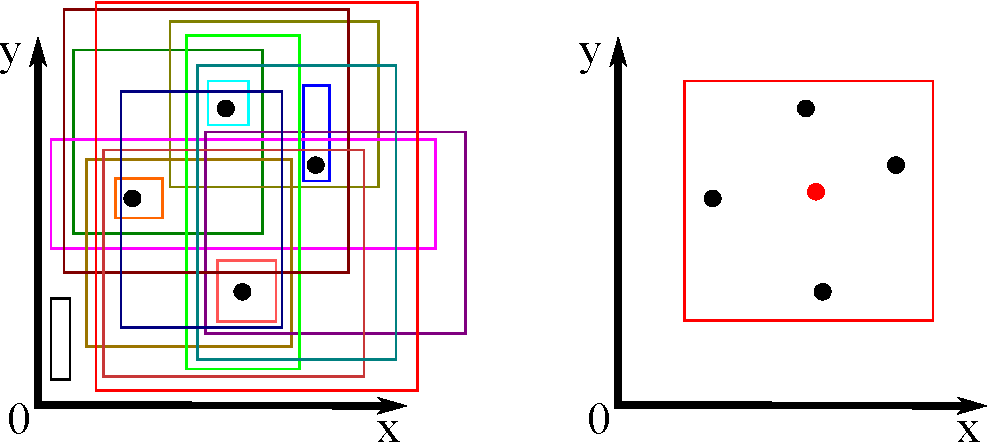
\includegraphics[width=.7\textwidth,keepaspectratio]{rectangles}
  \caption{Example of range set and VC-dimension. The domain is the
  plane $\mathbb{R}^2$ and the range set is the set of all
  \emph{axis-aligned rectangles}. The figure on the left shows graphically that
  it is possible to shatter a set of four points using 16 rectangles. On the
  right instead, one can see that it is impossible to shatter five points, as,
  for any choice of the five points, there will always be one (the red point in
  the figure) that is internal to the convex hull of the other four, so it would
  be impossible to find an axis-aligned rectangle containing the four points
  but not the internal one. Hence $\VC(\range)=4$.}
  \label{fig:rectangles}
\end{figure}

Given a probability distribution $\nu$ on the elements of $D$, the main
application of (empirical) VC-dimension in statistics and learning theory is in
computing the number of samples needed to approximate the probabilities
associated to the ranges through their empirical averages.  Formally, let
$X_1^k=(X_1,\dotsc,X_k)$ be a collection of independent identically distributed
random variables taking values in $D$, sampled according to $\nu$.
For a set $A\subseteq D$, let $\nu(A)$ be the probability that a sample from
$\nu$ belongs to the set $A$, and let
\[
\nu_{X_1^k}(A)=\frac{1}{k}\sum_{j=1}^k\mathds{1}_A(X_j),\]
where $\mathds{1}_A$ is the indicator function for $A$. The function
$\nu_{X_1^k}(A)$ is the \emph{empirical average} of $\nu(A)$ on $X_1^k$.

\begin{definition}\label{def:eapprox}
  Let $\range$ be a range set on a domain
  $D$ and $\nu$ be a probability distribution on $D$. For $\varepsilon\in(0,1)$,
  an \emph{$\varepsilon$-approximation to $(\range,\nu)$} is a bag $S$ of
  elements of $D$ such that
  \[
  \sup_{A\in\range}|\nu(A)-\nu_S(A)|\le\varepsilon\enspace.\]
\end{definition}

An $\varepsilon$-approximation can be constructed by sampling a sufficient
number of points of $D$ according to the distribution $\nu$, provided an upper
bound to the VC-dimension of $\range$ or to its empirical VC-dimension is known:

\begin{theorem}[Thm.~2.12~\citep{HarPS11}%, see also~\citep{LiLS01}
]\label{thm:eapprox}
  Let $\range$ be a range set on a domain
  $D$ with $\VC(\range)\le d$, and let $\nu$ be a distribution on $D$. Given
  $\delta\in(0,1)$ and a positive integer $\ell$, let
  \begin{equation}\label{eq:vceapprox}
    \varepsilon = \sqrt{\frac{c}{\ell}\left(d + \ln\frac{1}{\delta}\right)}
  \end{equation}
  where $c$ is an universal positive constant. Then, a bag of $\ell$
  elements of $D$ sampled \emph{independently} according to $\nu$ is an
  $\varepsilon$-approximation to $(\range,\nu)$ with probability at least
  $1-\delta$.
\end{theorem}
The constant $c$ is at most $0.5$~\citep{LofflerP09}.

%A similar result holds when an upper bound to the empirical VC-Dimension is
%available~\citep{BoucheronBL05}.
%\begin{theorem}[Sect.~3~\citep{BoucheronBL05}]\label{thm:eapproxempir}
%  Let $\range$ be a range set on a domain
%  $D$, and let $\nu$ be a distribution on $D$. Let
%  $X_1^\ell=(X_1,\dotsc,X_\ell)$ be a collection of elements from $D$ sampled
%  independently according to $\nu$. Let $d$ be an integer such that
%  $\EVC(\range,X_1^\ell)\le d$.
%  Given $\delta\in(0,1)$, let
%  \begin{equation}\label{eq:evceapprox}
%    \varepsilon =
%	2\sqrt{\frac{2d\log_2\frac{e\ell}{d}}{\ell}}+\sqrt{\frac{2\ln\frac{4}{\delta}}{\ell}}.
%  \end{equation}
%   Then, $X_1^\ell$ is a $\varepsilon$-approximation for $(\range,\nu)$
%   with probability at least $1-\delta$.
%\end{theorem}

The following theorem bounds the maximum deviation $\varepsilon$ in terms of
the empirical VC-dimension and of other sample-dependent quantities. We present
its proof in the Appendix.

\begin{theorem}\label{thm:eapproxempir}
	Let $\range$ be a range set on a domain $D$ and let $\nu$ be a distribution
	on $D$. Let $S$ be a collection of $\ell$ elements from $D$ sampled
	independently according to $\nu$, and let $\EVC(\range,S)\le d$. Given
	$\delta\in(0,1)$, let
	\begin{equation}\label{eq:evceapprox}
		\varepsilon = 2\max_{r\in\range}\sqrt{|r\cap
		S|}\frac{\sqrt{2\min\left\{\ln|\range|,d\ln\frac{en}{d}\right\}}}{\ell} +
		\sqrt{\frac{2\ln\frac{4}{\delta}}{\ell}}\enspace.
	\end{equation}
	Then $S$ is a $\varepsilon$-approximation for $(\range,\nu)$ with
	probability at least $1-\delta$.
\end{theorem}

%\subsection{Statistical hypothesis testing}\label{sec:stat_tests}
%We develope our methods to identify the True Frequent Itemsets within the
%framework of \emph{statistical
%hypothesis testing}. In statistical hypothesis testing, one uses some data
%$Y$ to evaluate a \emph{null hypothesis} $H$, whose rejection corresponds to claiming
%the identification of a significant phenomenon. A \emph{test statistic} $t_H(Y)$ associated
%to the hypothesis is computed from the data. If the $t_H(Y)$ belongs to a predefined
%\emph{acceptance region} (a subset of the domain of $t_H$), then $H$ is
%accepted, otherwise it is rejected. The acceptance region is defined a priori
%in such a way that the probability of a \emph{false positive}, i.e., the
%probability of accepting a true null hypothesis (corresponding to a non significant
%phenomenon), is at most some \emph{critical
%value} $\alpha$. Accepting a true null hypothesis is also called a ``Type-1
%error''. Often, defining an acceptance region as function of $\alpha$ is done
%implicitly, and instead of verifying whether the statistics belongs to it, one
%evaluates the associated \emph{$p$-value}, that is, the probability that the
%statistic $t_H$ is at least as extreme as the value observed on the given data,
%conditioning on the null hypothesis being true, and reject $H$ if the $p$-value
%is not larger than $\alpha$. Another important factor for a
%statistical test is its \emph{power}, that is the probability that the test
%correctly rejects the null hypothesis when the null hypothesis is false (also
%defined as $1-\Pr[\text{Type-2 error}]$, where a ``Type-2 error'' consists in
%non rejecting a false null hypothesis).
%
%In our scenario, the na\"{i}ve method to employ statistical hypothesis testing
%to find the TFIs is to define a null hypothesis $H_A$ for every itemset $A$,
%with $H_A =$ ``$\tfreq(A) < \theta$'', and to compute the $p$-value for such null
%hypothesis using $f_\Ds (A)$ as statistic. In particular, the $p$-value is given
%by the probability that the frequency of $A$ in a random dataset (with the same
%number of transactions of $\Ds$) sampled from $\prob$ is $\ge f_\Ds (A)$
%\emph{conditioning} on the event ``$\tfreq(A)< \theta$''. This is easy to
%compute given that the number of transactions in a dataset that contain $A$ has
%a Binomial distribution whose parameters are the size of the dataset and the
%true frequency of $A$ (\emph{Binomial test}). If the $p$-value is ``small enough'', the
%null hypothesis is rejected, that is $A$ is flagged as a TFI. The issue, in
%our case, is that we are considering a number of itemsets, that is we are facing a
%\emph{multiple hypothesis testing} problem~\cite{LiuZW11}. In this case, one is
%interested in controlling the probability of false discoveries among all the
%hypotheses tested, i.e., in controlling the \emph{Family-Wide Error Rate}.
%
%\begin{definition}\label{def:FWER}
%  The Family-Wise Error Rate (FWER) of a statistical test is the probability of reporting
%  at least one false discovery.
%\end{definition}
%
%In order to achieve the desired FWER, one must define a sequence of critical
%values for the individual hypotheses, that is, implicitly define a sequence of
%acceptance region for the test statistics. The \emph{Bonferroni
%correction}~\citep{DudoitSB03} is a widely-employed method to define such a
%sequence. In its simplest form, the Bonferroni correction suggests to compare
%the $p$-value of each hypothesis to the critical value $\alpha/m$, where $\alpha$ is the
%desired FWER, and $m$ is the number of hypotheses to be tested.  The Bonferroni
%correction is not a good choice to identify TFIs,
%%as it is known to be
%l%oose when the hypotheses are correlated, which is indeed the case
%fo%r TFIs.  Moreover,
%since the statistical power of methods that use the Bonferroni
%correction decreases with the number of hypotheses tested. In practical cases
%there would be hundreds or thousands of TFIs, making the use of the Bonferroni
%correction impractical if one wants to achieve high statistical power.

%If we were to use the same critical
%value $\alpha$ as in the single case, we could potentially produce a number
%of spurious discoveries~\cite{LiuZW11}. In order to avoid this issue, a multiple
%hypothesis correction is employed, like the Bonferroni
%correction~\citep{DudoitSB03} %(see Section~\ref{sec:statpow}).

%When only one hypothesis is considered,
%the null hypothesis is rejected when the $p$-value is at most $\alpha$, with
%$\alpha$ usually set to $0.05$ or $0.01$. This guarantees that the
%\emph{significance level}, that is the probability of incorrectly flagging an
%itemset as True Frequent (Type-1 error), is bounded by $\alpha$.

%In our scenario, since we are considering a number of itemsets, we are facing a
%\emph{multiple hypothesis testing} problem. If we were to use the same
%procedure as the single hypothesis case, we could potentially produce a number
%of spurious discoveries~\cite{LiuZW11}. In order to avoid this issue, a multiple
%hypothesis correction is employed, like the Bonferroni
%correction~\citep{DudoitSB03} %(see Section~\ref{sec:statpow}).

%\begin{definition}\label{def:FWER}
%  The Family-Wise Error Rate (FWER) of a statistical test is the probability that at
%  least one false positive is reported as significant.
%\end{definition}

%The Bonferroni correction guarantees that the FWER is bounded by $\alpha$.  A
%recently proposed alternative to  bound the FWER is to bound the False Discovery
%Rate (FDR), that in our case correspond to the proportion of false discoveries
%among the TFI. The use of the FDR allows to produce in output a larger number of
%patterns, since a small proportion of false discoveries are tolerated in the output;
%however, in frequent itemset mining mining the number of patterns produced is usually high,
%therefore having a smaller number of high quality discoveries is preferable to
%reporting a larger number of patterns containing some false discoveries.

%\iffalse
%\begin{definition}\label{def:FDR}
% The False Discovery Rate~\citep{BenjaminiH95} (FDR) is the expected proportion of
% false positives among all itemsets that are reported as significant.
%\end{definition}
%\fi

%We focus in this work on identifying a highly reliable collections of high
%quality itemsets, and therefore aim to identify True Frequent Itemsets while
%bounding the FWER of our method, that is we bound the probability that the
%collection of itemsets reported by our method contains \emph{any} spurious
%discovery (any itemeset that is not True Frequent)
%
%Another important factor for a statistical test is its \emph{power}, that is the
%probability that the test correctly rejects the null hypothesis when the null
%hypothesis is false (also defined as $1-\Pr[\text{Type-2 error}]$).


\section{The range set of a collection of itemsets}\label{sec:range}
In this section we define the concept of a range set associated to a
collection of itemsets and show how to bound the VC-dimension and the
empirical VC-dimension of this range set. We use these definitions and results
to develop our algorithm in later sections.

\begin{definition}\label{def:rangeset}
Given a collection $\mathcal{C}$ of itemsets built on a ground set $\Itm$, the
\emph{range set $\range(\mathcal{C})$ associated to $\mathcal{C}$ is a range
set on $2^\Itm$} containing the support sets of the itemsets in $\mathcal{C}$:
\[\range(\mathcal{C})=\{T(A) ~:~ A\in\mathcal{C}\}\enspace.\]
\end{definition}

\begin{fact}\label{fact:maxfreq}
	Given this definition and a dataset $\Ds$, the maximum
	from~\eqref{eq:evceapprox} is attained for the item $a\in\Itm$ with the
	highest frequency in $\Ds$, and the value of $|r\cap S|$ is exactly
	$f_\Ds(\{a\})|\Ds|$.
\end{fact}

The following Theorem presents an upper bound to the empirical VC-dimension of
$\range(\mathcal{C})$ on a dataset $\Ds$.

\begin{theorem}\label{lem:evcdimupbound}
  Let $\mathcal{C}$ be a collection of itemsets and let $\Ds$ be a dataset. Let
  $d$ be the maximum integer for which there are at least $d$
  transactions $\tau_1,\dotsc,\tau_d\in \Ds$ such that the set
  $\{\tau_1,\dotsc,\tau_d\}$ is an \emph{antichain}\footnote{An antichain is a
  collection of sets such no one of them is a subset of another.}, and each $\tau_i$, $1\le i\le d$,
  contains at least $2^{d-1}$ itemsets from $\mathcal{C}$.
  %\begin{enumerate*}
  %  \item
  %    The set $\{\tau_1,\dotsc,\tau_d\}$ is an antichain, and
  %    %For any pair of transactions $(\tau_i,\tau_j)$, $i\neq j$, we have
  %    %$\tau_i\not\subseteq\tau_j$ and $\tau_j\not\subseteq\tau_i$, and
  %  \item Each $\tau_i$, $1\le i\le d$ contains at least $2^{d-1}$ itemsets from
  %    $\mathcal{C}$.
  %\end{enumerate*}
  Then $\EVC(\range(\mathcal{C}),\Ds)\le d$.
\end{theorem}

\begin{proof}
  The antichain requirement guarantees that the set of transactions considered in
  the computation of $d$ could indeed theoretically be shattered. Assume that a
  subset $\mathcal{F}$ of $\Ds$ contains two transactions $\tau'$ and $\tau''$
  such that $\tau'\subseteq\tau''$. Any itemset from $\mathcal{C}$
  appearing in $\tau'$ would also appear in $\tau''$, so there would not be any
  itemset $A\in\mathcal{C}$ such that $\tau''\in T(A)\cap F$ but
  $\tau'\not\in T(A)\cap \mathcal{F}$, which would imply that $\mathcal{F}$ can
  not be shattered. Hence sets that are not antichains should not be
  considered. This has the net effect of potentially resulting in a lower $d$,
  i.e., in a stricter upper bound to $\EVC(\range(\mathcal{C}),\Ds)$.

  Let now $\ell>d$ and consider a set $\mathcal{L}$ of $\ell$ transactions from
  $\Ds$ that is an antichain. Assume that $\mathcal{L}$ is shattered by
  $\range(\mathcal{C})$. Let $\tau$ be a transaction in $\mathcal{L}$.
  The transactions $\tau$ belongs to $2^{\ell-1}$ subsets of $L$. Let
  $\mathcal{K}\subseteq \mathcal{L}$ be one of these subsets. Since
  $\mathcal{L}$ is shattered, there exists an itemset $A\in\mathcal{C}$ such
  that $T(A)\cap \mathcal{L}=\mathcal{K}$. From this and the fact
  that $t\in \mathcal{K}$, we have that $\tau\in T(A)$ or equivalently that
  $A\subseteq\tau$. Given that all the subsets $\mathcal{K}\subseteq\mathcal{L}$
  containing $\tau$ are different, then also all the $T(A)$'s such that
  $T(A)\cap \mathcal{L}=\mathcal{K}$ should be
  different, which in turn implies that all the itemsets
  $A$ should be different and that they should all appear in $\tau$. There are
  $2^{\ell-1}$ subsets $\mathcal{K}$ of $\mathcal{L}$ containing $\tau$,
  therefore $\tau$ must contain at least $2^{\ell-1}$ itemsets from
  $\mathcal{C}$, and this holds for all $\ell$ transactions in $\mathcal{L}$. This is a
  contradiction because $\ell>d$ and $d$ is the
  maximum integer for which there are at least $d$ transactions containing at
  least $2^{d-1}$ itemsets from $\mathcal{C}$. Hence $\mathcal{L}$ cannot be shattered and
  the thesis follows.
\end{proof}

\subsection{Computing the VC-Dimension}\label{sec:computvc}
The na\"ive computation of $d$  according to the definition in Thm.~\ref{lem:evcdimupbound}
requires to scan the transactions one by one,
compute the number of itemsets from $\mathcal{C}$ appearing in each
transaction, and make sure to consider only itemsets constituting antichains. Given the very large
number of transactions in typical dataset and the fact that the number of
itemsets in a transaction is exponential in its length, this method would be
computationally too expensive. An upper bound to $d$ (and therefore to
$\EVC(\range(\mathcal{C}),\Ds)$) can be computed by solving a
\emph{Set-Union Knapsack Problem} (SUKP)~\citep{GoldschmidtNY94} associated to
$\mathcal{C}$.
%where the elements to be put in the knapsack are organized into sets, which have a profit associated to them. The objective is to maximize
%the number of sets for which all the elements in those
%sets were put in the knapsack
%the profit, while satisfying the capacity constraint.

\begin{definition}[\citep{GoldschmidtNY94}]\label{def:sukp}
  Let $U=\{a_1,\dotsc,a_\ell\}$ be a set of elements and let
  $\mathcal{S}=\{A_1,\dotsc,A_k\}$ be a set of subsets of $U$, i.e.
  $A_i\subseteq U$ for $1\le i\le k$. Each subset $A_i$, $1\le i\le k$, has an associated
  non-negative \emph{profit} $\rho(A_i)\in\mathbb{R}^+$, and each element $a_j$, $1\le
  j\le\ell$ as an associated non-negative weight $w(a_j)\in\mathbb{R}^+$.
  Given a subset $\mathcal{S}'\subseteq\mathcal{S}$, we define the profit of
  $\mathcal{S}'$ as $P(\mathcal{S}')=\sum_{A_i\in \mathcal{S}'}\rho(A_i)$. Let
  $U_{\mathcal{S}'}=\cup_{A_i\in\mathcal{S}'} A_i$. We
  define the weight of $\mathcal{S}'$ as $W(\mathcal{S}')=\sum_{a_j\in
  U_{\mathcal{S}'}} w(a_j)$. Given a non-negative parameter $c$ that we call
  \emph{capacity}, the \emph{Set-Union Knapsack Problem} (SUKP) requires to find
  the set $\mathcal{S}^*\subseteq\mathcal{S}$ which \emph{maximizes}
  $P(\mathcal{S}')$ over all sets $\mathcal{S}'$ such that $W(\mathcal{S}')\le c$.
\end{definition}

In our case, $U$ is the set of items that appear in the itemsets of
$\mathcal{C}$, $\mathcal{S}=\mathcal{C}$, the profits and the weights are all
unitary, and the capacity constraint is an integer $\ell$. We call this
optimization problem the \emph{SUKP associated to $\mathcal{C}$ with capacity
$\ell$}.
It is easy to see %It should be evident
that the optimal profit of this SUKP is the maximum number
of itemsets from $\mathcal{C}$ that a transaction of length $\ell$ can contain.  %could fit into a transaction of length %$\ell$.
In order to show how to use this fact to compute an upper bound to
$\EVC(\range(\mathcal{C}),\Ds)$, we need to define some additional terminology. Let
$\ell_1,\dotsc,\ell_w$ be the sequence of the
\emph{transaction lengths} of $\Ds$, i.e., for each value $\ell$
for which there is at least a transaction in $\Ds$ of length $\ell$, there is
one (and only one) index $i$, $1\le i\le w$ such that $\ell_i=\ell$. Assume that
the $\ell_i$'s are labelled in sorted decreasing order:
$\ell_1>\ell_2>\dotsb>\ell_w$. Let now $L_i$, $1\le i\le w$ be the maximum number of
transactions in $\Ds$ that have length at least $\ell_i$ and such that
for no two $\tau'$, $\tau''$ of them we have either $\tau'\subseteq\tau''$ or
$\tau''\subseteq\tau'$. Let now $q_i$ be the optimal profit of the SUKP associated to
$\mathcal{C}$ with capacity $L_i$, and let $b_i=\lfloor \log_2q_i\rfloor +1$.
The sequences $(\ell_i)_1^w$ and a sequence $(L_i^*)^w$ of upper bounds to
$(L_i)_1^w$ can be computed efficiently with a scan of the dataset.
The following lemma uses these sequences to show how to obtain an upper bound to
the empirical VC-dimension of $\mathcal{C}$ on $\Ds$.

\begin{lemma}\label{lem:sukpevc}
  Let $j$ be the minimum integer for which $b_i\le L_i$. Then
  $\EVC(\mathcal{C},\Ds)\le b_j$. %We call $b_j$ the \emph{empirical b-index of
  %$\mathcal{C}$ on $\Ds$} and denote it as $\eb(\mathcal{C},\Ds)$
\end{lemma}
\begin{proof}
  If $b_j\le L_j$, then there are at least $b_j$ transactions which can contain
  $2^{b_j-1}$ itemsets from $\mathcal{C}$ and this is the maximum $b_i$ for
  which it happens, because the sequence $b_1,b_2,\dotsc,b_w$ is sorted in
  decreasing order, given that the sequence $q_1,q_2,\dotsc,q_w$ is. Then $b_j$
  satisfies the conditions of Lemma~\ref{lem:evcdimupbound}. Hence
  $\EVC(\mathcal{C},\Ds)\le b_j$.
\end{proof}

\begin{corollary}\label{lem:sukpvc}
  Let $q$ be profit of the SUKP associated to $\mathcal{C}$ with capacity
  equal to $\ell=|\{a\in\Itm ~:~ \exists A\in\mathcal{C} \mbox{ s.t. } a\in
  A\}|$ ($\ell$ is the number of items such that there is at least one itemset in $\mathcal{C}$ containing
  them).
  %$|\Itm|-1$.
  Let $b=\lfloor\log_2 q\rfloor + 1$. Then
  $\VC(\range(\mathcal{C}))\le b$. %We call $b*$ the \emph{b-index of
  %$\mathcal{C}$} and denote it as $\b(\mathcal{C})$.
\end{corollary}

\paragraph{Complexity and runtime considerations.} Solving the SUKP optimally is
NP-hard in the general case, although there are known restrictions for
which it can be solved in polynomial time using dynamic
programming~\citep{GoldschmidtNY94}. Since we have unit weights and unit
profits, our SUKP is equivalent to the \emph{densest $k$-subhypergraph} problem,
which can not be approximated within a factor of $2^{O(\log n)^\delta}$ for any
$\delta>0$ unless $3STA \in
DTIME(2^{n^{3/4+\varepsilon}})$~\citep{HajiaghayiJKLMRSV06}. A greedy algorithm
by~\citet{Arulselvan14} allows a constant factor approximation if each
items only appear in a constant fraction of itemsets of $\mathcal{C}$.
%It is not clear whether our case falls into
%one of these restrictions but we found that
For our case, it is actually \emph{not necessary to compute the optimal
solution} to the SUKP: any upper bound solution for which we can prove that
there is no power of two between that solution and the optimal solution would
result in the \emph{same upper bound} to the (empirical) VC-dimension, while
substantially speeding up the computation. This property can be specified in
currently available optimization problem solvers (e.g., CPLEX), which can then can compute the
bound to the (empirical) VC-dimension very fast even for very large instances
with thousands of items and hundred of thousands of itemsets in $\mathcal{C}$,
making this approach practical.

\paragraph{Refinements.} It is possible to make some refinements to our
computation of the \emph{empirical} VC-dimension of a collection $\mathcal{C}$ of
itemsets on a dataset $\Ds$. First of all, one can remove from $\mathcal{C}$ all
itemsets that never appear in $\Ds$, as the corresponding ranges can not help
shattering any set of transactions in $\Ds$. Identifying which itemsets to
remove requires a single linear scan of $\Ds$. Secondly, when computing the
capacities $L_i$ (i.e., their upper bounds $L_i^*$), we can ignore all the
transactions that do not contain \emph{any} of the itemsets in $\mathcal{C}$ (or
the filtered version of $\mathcal{C}$), as there is no way of shatter them using
the ranges corresponding to itemsets in $\mathcal{C}$. Both refinements aim at
reducing the optimal value of the SUKP associated to $\mathcal{C}$, and
therefore at computing a smaller bound to the empirical VC-dimension of
$\mathcal{C}$ on $\Ds$. We remark that these refinements can not be used when
computing the (non-empirical) VC-dimension.

\paragraph{The range set of all itemsets.}
The range set associated to $2^\Itm$
is particularly interesting for us. It is possible  %It is easy
to compute bounds to $\VC(\range(2^\Itm))$ and
$\EVC(\range(2^\Itm), \Ds)$ without having to solve a SUKP.
%\citet{RiondatoU12} gave an upper bound to the empirical VC-dimension of
%$\range(2^\Itm)$ on $\Ds$.
%Before presenting the bound, we need to introduce a
%characteristic quantity of the set of transactions $\Ds$ called the \emph{d-index} and
%denoted as $\mathsf{d}(\Ds)$.

%\begin{definition}\label{def:dindex}
\begin{theorem}[\citep{RiondatoU12}]\label{thm:empvcdimubfirst}
  Let $\Ds$ be a dataset built on a
  ground set $\Itm$. The
  \emph{d-index} $\mathsf{d}(\Ds)$ of $\Ds$ is the maximum integer $d$ such that
  $\Ds$ contains at least $d$ transactions of length at least $d$ %such that
  %no one of them is a subset of another, that is, they form an antichain
  that form an antichain. %
  %for any two of these transactions $\tau',\tau''$ we have neither $\tau'\subseteq
  %\tau''$ nor $\tau''\subseteq \tau'$.
  We have $\EVC(\range(2^\Itm),\Ds)\le \mathsf{d}(\Ds)$.
%\end{definition}
\end{theorem}

%\citet{RiondatoU12} presents an efficient algorithm to compute an upper bound to
%the d-index of a dataset with a single linear scan of the dataset $\Ds$.

%\begin{theorem}\label{thm:empvcdimubfirst}
%  \emph{(\citep[Thm.~3]{RiondatoU12})} Let $\Ds$ be a dataset  with
%  transactions built on a ground set $\Itm$. Then $\EVC(\range(2^\Itm),\Ds)\le
%  \mathsf{d}(\Ds)$.
%\end{theorem}

%It easy to extend this theorem to prove an upper bound to the VC-dimension of
%$\range(2^\Itm)$.
\begin{corollary}\label{thm:vcdimubfirst}
  %Let $\Ds$ be a dataset with transactions built on a ground set $\Itm$. Then
  $\VC(\range(2^\Itm))\le |\Itm|-1$.
\end{corollary}
%\begin{proof}
%  Let $k=|\Itm|$. Assume w.l.o.g.~that $\Itm=\{1,\dotsc,k\}$. Let
%  $\tau_i=\Itm\setminus\{i\}$, $1\le i\le k$. We have $|\tau_i|=k-1$, for $1\le
%  i\le k$. Notice that for $i\neq j$, neither $\tau_i\subseteq\tau_j$ nor
%  $\tau_j\subseteq\tau_i$. Consider a dataset $\Ds$ made of the set of
%  transactions $\{\tau_1,\dotsc,\tau_k\}$ and any number of additional
%  transactions. It is easy to see that $\mathsf{d}(\Ds)=k-1$, and that
%  it is impossible to build a dataset with a larger d-index using the items of
%  $\Itm$, because there is no way to use the items of $\Itm$ to build $\ell>k-1$
%  transactions of length at least $\ell$ and such that for any two of these
%  transactions $\tau',\tau''$ we have neither $\tau'\subseteq \tau''$ nor
%  $\tau''\subseteq \tau'$. This concludes the proof. \qed
%\end{proof}

\citet{RiondatoU12} presented an efficient algorithm to compute an upper bound to
the d-index of a dataset with a single linear scan of the dataset $\Ds$.
The upper bound presented in Thm.~\ref{thm:empvcdimubfirst} is tight:
%, in the sense that
 there are datasets for which
$\EVC(\range(2^\Itm),\Ds)=\mathsf{d}(\Ds)$~\citep{RiondatoU12}.
This implies that the upper bound presented in Corol.~\ref{thm:vcdimubfirst} is
also tight.

%The upper bound to the empirical VC-Dimension of $\range(2^\Itm)$ on $\Ds$ is used
%by~\citet{RiondatoU12} to compute the size of a sample $\Sam$ needed to extract
%a superset of the collection of $\FI(\Ds,\Itm,\theta)$ from $\Sam$, where the
%quality of the approximation is controlled by user-defined parameters
%$\varepsilon$ and $\delta$. In this work we will use the two upper bounds
%presented above to compute a superset of the negative border of the collection
%of RFI's with respect to a minimum real frequency threshold $\theta$.


\section{Finding the True Frequent Itemsets}\label{sec:main}
In this section we present an algorithm that receives in input a dataset $\Ds$,
a minimum frequency threshold $\theta$, and a confidence parameter
$\delta\in(0,1)$ and identifies a threshold $\hat{\theta}$ such that, with
probability at least $\delta$, all itemsets with frequency at least
$\hat{\theta}$ in $\Ds$ are True Frequent Itemsets with respect to $\theta$. The
threshold $\hat{\theta}$ can be used to find a collection
$\mathcal{C}=\FI(\Ds,\Itm,\hat\theta)$ of itemsets such that $\Pr(\exists
A\in\mathcal{C} \mbox{ s.t.~} \tfreq(A)<\theta)<\delta$.

%It starts by building a set
%$\mathcal{G}$ of ``candidates TFIs''. For each itemset
%$A\in\mathcal{G}$ we evaluate the probability that $\tfreq(A)$ is less than $\theta$
%by considering the probability that  $f(A)$ of $A$ in
%the dataset is observed when $\tfreq(A) < \theta$. If
%the frequency falls into the \emph{acceptance region} %$\Delta=[0,\theta+\varepsilon)$
%$[0,\theta+\varepsilon)$, where $\varepsilon$ is a function of $\delta$ and
%$\mathcal{G}$ computed by our methods,
%then $H_A$ is \emph{accepted}, otherwise $H_A$ is \emph{rejected}
%and $A$ is flagged as True Frequent and included in the output collection
%$\mathcal{C}$. Any
%itemset not in $\mathcal{G}$ is not considered and will not
%be reported in output. It should be clear that the definition of the acceptance
%region is critical for the method to have the desired FWER at most
%$\delta$: one needs to compute an $\varepsilon$ such that
%\[
%\Pr\left(\exists A\in\mathcal{C}\mbox{ s.t. }
%\tfreq(A)<\theta\right)=\Pr\left(\exists A\in\mathcal{G} \mbox{ s.t. }
%\tfreq(A)<\theta \mbox{ and }
%f(A)\ge\theta+\varepsilon\right)\le\delta\enspace.\]


%The two methods we present differ in the definition of $\mathcal{G}$ and in the
%computation of $\varepsilon$, but both use the tools we developed in
%Sect.~\ref{sec:range}.


%\subsection{An holdout approach}\label{sec:holdout}

{\bf PER MATTEO: } Sistema questa sezione dopo gli ultimi stravolgimenti

We now present and analyze a second method, called \ALGHOLDOUT, for
mining the TFIs. \ALGHOLDOUT draws inspiration from the holdout technique
presented by~\citet{Webb07}, and requires that the dataset $\Ds$ can be
randomly split into two parts that do not need to be of the same size, but
it \emph{must} be possible to see them as two independent collections of
i.i.d.~samples from the generating distribution $\pi$: an \emph{exploratory}
part $\Ds_\mathrm{e}$ and an \emph{evaluation} part $\Ds_\mathrm{v}$.
\ALGHOLDOUT works in two phases: we first use the exploratory part
$\Ds_\mathrm{e}$ to identify a small set $\mathcal{G}$ of candidate TFIs, and
then we decide which of the candidates to include in the output using their
frequencies in the evaluation part $\Ds_\mathrm{v}$.

\paragraph{First phase.} Let $\delta_\mathrm{e}$ and $\delta_\mathrm{v}$ be such
that $(1-\delta_\mathrm{e})(1-\delta_\mathrm{v})\ge(1-\delta)$. Let
$\range(2^\Itm)$ be the range space of all itemsets. We can compute an upper
bound $d'$ to $\VC(\range(2^\Itm))$ and an upper bound $d''$ to
$\EVC(\range(2^\Itm),\Ds_\mathrm{e})$, using respectively
Corol.~\ref{thm:vcdimubfirst} and Thm.~\ref{thm:empvcdimubfirst}). Then, given
that $\Ds_\mathrm{e}$ is a collection of i.i.d.~samples from the generative
distribution $\prob$, we can use $d'$ in Thm.~\ref{thm:eapprox} (resp.~$d''$ in
Thm~\ref{thm:eapproxempir}) to compute an $\varepsilon_\mathrm{e}'$ (resp.~an
$\varepsilon_\mathrm{e}''$) such that $\Ds_\mathrm{e}$ is, with probability at
least $1-\delta_1$, an $\varepsilon_\mathrm{e}'$-approximation
(resp.~$\varepsilon_\mathrm{e}''$-approximation) to $(\range(2^\Itm),\prob)$.
Then, if we let
$\varepsilon_\mathrm{e}=\min\{\varepsilon_\mathrm{e}',\varepsilon_\mathrm{e}''\}$,
we have that $\Ds_\mathrm{e}$ is, with probability at least $1-\delta_1$, an
$\varepsilon_\mathrm{e}$-approximation to $(\range(2^\Itm),\prob)$. These steps
are exactly the same as the first steps of \ALG, which operated on the
\emph{whole} dataset, not just on one part like \ALGHOLDOUT. We then compute the
collections of itemsets $\mathcal{C}_\mathrm{e}=\{X\subseteq\Itm ~:~
f_{\Ds_\mathrm{e}}(X)\ge\theta+\varepsilon_\mathrm{e}\}$ and
$\mathcal{G}=\{X\subseteq\Itm ~:~ \theta\le
f_{\Ds_\mathrm{e}}(X)<\theta+\varepsilon_\mathrm{e}\}$. To obtain these sets, we
extract the set $\FI(\Ds_\mathrm{e},\Itm,\theta)$ and partition it appropriately
into $\mathcal{C}_\mathrm{e}$ and $\mathcal{G}$.

\paragraph{Second phase.} In the second phase, we compute a value
$\varepsilon_\mathrm{v}$ such that, with probability at least $1-\delta_2$, the
evaluation dataset $\Ds_\mathrm{v}$ is an $\varepsilon_\mathrm{v}$-approximation
to $(\range(\mathcal{G}),\prob)$. In
order to obtain $\varepsilon_\mathrm{v}$ through
Thms.~\ref{thm:eapprox} and~\ref{thm:eapproxempir}, we need to compute upper
bounds to $\VC(\range(\mathcal{G}))$ and
$\EVC(\range(\mathcal{G}),\Ds_\mathrm{v})$. We solve SUKPs associated to
$\mathcal{G}$ and obtain such bounds, as stated in Lemma~\ref{lem:sukpevc}
respectively. We then use these bounds and Thm.~\ref{thm:eapprox}
(resp.~Thm.~\ref{thm:eapproxempir}) to compute a
$\varepsilon_\mathrm{v}'$ (resp.~ $\varepsilon_\mathrm{v}''$) such that
$\Ds_\mathrm{v}$ is, with probability at least $1-\delta_2$, an
$\varepsilon_\mathrm{v}'$-approximation (resp.~an
$\varepsilon_\mathrm{v}''$-approximation) to $(\range(\mathcal{G}),\prob)$. Once
we have obtained
$\varepsilon_\mathrm{v}=\min\{\varepsilon_\mathrm{v}',\varepsilon_\mathrm{v}''\}$,
we compute the set
\[
\mathcal{C}_\mathrm{v}=\{X\subseteq\Itm ~:~ X\in\mathcal{G} \mbox{ and }
f_{\Ds_\mathrm{v}}(X)\ge\theta+\varepsilon''\}=\mathcal{G}\cap\FI(\Ds_\mathrm{v},\Itm,\theta+\varepsilon_\mathrm{v}).\]
The method returns the collection of itemsets $\mathcal{C}_\mathrm{e}\cup\mathcal{C}_\mathrm{v}$.
%The proof that $\Pr(\exists
%A\in\mathcal{C}_\mathrm{e}\cup\mathcal{C}_\mathrm{v} \mbox{ s.t. }
%\tfreq(A)<\theta)\le\delta$ comes from the definition of $\varepsilon_\mathrm{e}$ and
%$\varepsilon_\mathrm{v}$ through Thms.~\ref{thm:eapprox}
%and~\ref{thm:eapproxempir}

\begin{theorem}
	With probability at least $1-\delta$,
	$\mathcal{C}_\mathrm{e}\cup\mathcal{C}_\mathrm{v}$ contains no false
	positives:
	\[
		\Pr(\exists A\in\mathcal{C}_\mathrm{e}\cup\mathcal{C}_\mathrm{v} \mbox{
		s.t. } \tfreq(A)<\theta)\le\delta\enspace.
	\]
\end{theorem}
\begin{proof}
  Consider the two events $\mathsf{E}_\mathrm{e}$=``$\Ds_\mathrm{e}$ is an
  $\varepsilon_\mathrm{e}$-approximation for $(\range(2^\Itm),\prob)$'' and
  $\mathsf{E}_\mathrm{v}=$``$\Ds_\mathrm{v}$ is an
  $\varepsilon_\mathrm{v}$-approximation for $(\range(\mathcal{G}),\prob)$. From
  the above discussion it follows that the event
  $\mathsf{E}=\mathsf{E}_\mathrm{e}\cap\mathsf{E}_\mathrm{v}$ occurs with probability at least
  $1-\delta$. Suppose from now on that indeed $\mathsf{E}$ occurs.

  Given that $\mathsf{E}_\mathrm{e}$ occurs, then all the itemsets with
  frequency in $\Ds_\mathrm{e}$ at least $\theta+\varepsilon_\mathrm{e}$
  must have a real frequency at least $\theta$. This equals to say that all
  itemsets in $\mathcal{C}_\mathrm{e}$ are True Frequent Itemsets
  ($\mathcal{C}_\mathrm{e}\subseteq TFI(\theta)$.

  Given that $\mathsf{E}_\mathrm{v}$ occurs, then we know that all itemsets in
  $\mathcal{G}$ have frequency in $\Ds_\mathrm{v}$ that is at most
  $\varepsilon_\mathrm{v}$ far from their true frequency:
  \[
  \max_{A\in\mathcal{G}}\left|\tfreq(A)-f_{\Ds_\mathrm{v}}(A)\right|\le\varepsilon_\mathrm{v}\enspace.\]
  In particular this means that an  itemset $A\in\mathcal{G}$ can have
  $f_{Ds_\mathrm{v}}(A)\ge\theta+\varepsilon_\mathrm{v}$ \emph{only} if
  $\tfreq(A)\ge\theta$, that is \emph{only} if $A\in\TFI(\prob,\Itm,\theta)$.
  Hence, $\mathcal{C}_\mathrm{v}\subseteq TFI(\prob,\Itm,\theta)$.

  We can then conclude that if the event $\mathsf{E}$ occurs, we have
  $\mathcal{C}_\mathrm{e}\cup \mathcal{C}_\mathrm{v}\subseteq TFI(\prob,\Itm,\theta)$.
  Since $\mathsf{E}$ occurs with probability at least $1-\delta$, this equals to
  say that
  \[
  \Pr(\exists A\in \mathcal{T}_\mathrm{e}\cup
  \mathcal{T}_\mathrm{v} ~:~ \tfreq(A)<\theta)\le\delta\enspace.\]
\end{proof}

{\bf MATTEO:} Pseudocodice, menzione dell'algoritmo in giro per il paper,
risultati sperimentali, etc.

The intuition behind the method is the following. Let $\mathcal{B}$ be the
\emph{negative border} of $\TFI(\prob,\Itm,\theta)$, that is the set of itemsets
not in $\TFI(\prob,\Itm,\theta)$ but such that all their proper subsets are in
$\TFI(\prob,\Itm,\theta)$. If we can find an $\varepsilon$ such that $\Ds$ is an
$\varepsilon$-approximation to $(\range(\mathcal{B}),\pi)$ then we have that any
itemset $A\in\mathcal{B}$ has a frequency $f_\Ds(A)$ in $\Ds$ less than
$\hat{\theta}=\theta+\varepsilon$, given that it must be $\tfreq(A)<\theta$. By
the antimonotonicity property of the frequency, the same holds for all itemsets
that are supersets of those in $\mathcal{B}$. Hence, the only itemsets that can
have frequency in $\Ds$ greater or equal to $\hat{\theta}=\theta+\varepsilon$
are those with true frequency at least $\theta$. In the following paragraphs we
show how to compute $\varepsilon$.

\paragraph{Computing a superset of $\mathcal{B}$.} The first step of our
algorithm, which we call \ALG{}, is to compute a superset of $\mathcal{B}$, the
negative border of $\TFI(\prob,\Itm,\theta)$. Let $\delta_1$ and $\delta_2$ be
such that $(1-\delta_1)(1-\delta_2)\ge 1-\delta$. Let $\range(2^\Itm)$ be the
range space of all itemsets. Let $d$ be the upper bound to the empirical
VC-dimension of $\range(2^\Itm)$ on $\Ds$, computed as discussed in
Sect.~\ref{sec:computvcexact}. We can then use~\eqref{eq:evceapproxitemsets}
with $\delta_1$, the bound $d$, and the maximum frequency of an item in $\Ds$ to
compute an $\varepsilon_1$ such that $\Ds$ is, with probability at least
$1-\delta_1$, an $\varepsilon_1$-approximation to $(\range(2^\Itm),\prob)$. Let
now $\mathcal{W}$ be the \emph{negative border} of
$\mathcal{C}_1=\FI(\Ds,\Itm,\theta-\varepsilon_1)$, and let
$\mathcal{G}=\{A\subseteq\Itm ~:~ \theta-\varepsilon_1\le
f_\Ds(A)<\theta+\varepsilon_1\}$, and $\mathcal{F}=\mathcal{G}\cup\mathcal{W}$.

\begin{fact}\label{fact:supersetborder}
	If $\Ds$ is a $\varepsilon_1$-approximation to $(\range(2^\Itm),\prob)$,
	then $\mathcal{B}\subseteq\mathcal{F}$.
\end{fact}

\paragraph{Computing an upper bound to $\EVC(\mathcal{B},\Ds)$.} Now that we
have a superset $\mathcal{F}$ of $\mathcal{B}$, we want to compute an upper
bound to the empirical VC-dimension of $\mathcal{B}$ on $\Ds$. Na\"ively, we
could use any of the algorithms presented in Sect.~\ref{sec:computvc} to compute
an upper bound to $\EVC(\mathcal{F},\Ds)$ and this would be a valid upper bound
to $\EVC(\mathcal{B},\Ds)$ (provided Fact~\ref{fact:supersetborder} holds). The
downside of this line of action is that $\mathcal{F}$ may be much larger than
$\mathcal{B}$ and, even more importantly, that we are choosing to ignore
available information on the structure of $\mathcal{B}$. In particular, we are
choosing to ignore the following.

\begin{fact}
	The negative border of a collection of itemsets is a \emph{maximal
	antichain} on $2^\Itm$
\end{fact}

The collection $\mathcal{F}$ is in general not an antichain, except for
degenerate and unrealistic cases. An upper bound to $\EVC(\mathcal{F},\Ds)$
would be a gross overestimation of $\EVC(\mathcal{B},\Ds)$, hence we would like
to incorporate the fact that $\mathcal{B}$ is a maximal antichain in our
computation of the bound to its empirical VC-dimension.

We can modify \texttt{EVCBoundExact} by including, after having computed the
set $\mathcal{C}_\tau$ (line~\ref{algline:intersectionloopend} in
Alg.~\ref{alg:evcboundexact}), the size $\ell_\tau$ of the largest antichain in
$\mathcal{C}_\tau$, which can be done in time polynomial in $\mathcal{C}_\tau$.
We can then use $\ell_\tau$ as the value for $L[I_\tau]$
(line~\ref{algline:assignmentintersection}). Since $\ell_\tau$ is the size of
the largest antichain in $\mathcal{C}_\tau$, then $\ell_\tau$ is an upper bound
to the number of itemsets from $\mathcal{B}$ that appear in $\tau$. Provided
that $\Ds$ is a $\varepsilon_1$-approximation to $(\range(2^\Itm),\prob)$ (so
that Fact~\ref{fact:supersetborder} holds) the so-modified algorithm, which we
call \texttt{EVCBoundAntichain}, clearly gives an upper-bound to the d-index of
$\mathcal{B}$ on $\Ds$, and therefore to $\EVC(\mathcal{B},\Ds)$. Due to the
additional computation of $\ell_\tau$, this algorithm is slower than
$\texttt{EVCBoundExact}$. It is possible to modify the second part of
\texttt{EVCBoundAntiChain} in the same way as \texttt{EVCBoundExact} was
modified to obtain \texttt{EVCBoundScan}, and obtain a slightly faster
algorithm. Nevertheless, we believe that the need to compute potentially for
each transaction $\tau$ both the set of itemsets of $\mathcal{C}$ in $\tau$ and
additionally the size of the largest antichain on this set, make using
\texttt{EVCBoundAntichain} a bit unpractical, despite being a polynomial time
algorithm.

It is actually for this reason that we developed \texttt{EVCBoundSUKP}, which we
can modify \texttt{EVCBoundSUKP} to solve a slightly modified SUKPs associated
to $\mathcal{F}$ with the \emph{additional constraint} that the optimal solution
(a collection of itemsets) \emph{must be a maximal antichain}. The correctness
follows from the fact that the optimal profit of the so-modified SUKP with
capacity $\ell$ is the maximum number of itemsets forming an antichain in
$\mathcal{F}$ that can be built using a subset of $\ell$ of $U$, so it is an
upper bound to the number of itemsets in $\mathcal{B}$ that can be built on
$\ell$ items of $U$, provided that $\Ds$ is a $\varepsilon_1$-approximation to
$(\range(2^\Itm),\prob)$ (so that Fact~\ref{fact:supersetborder} holds). Hence
Lemma~\ref{lem:sukpevc} carries over and this new algorithm, called
\texttt{EVCBoundSUKPAntiChain} is correct. This algorithm is more practical than
\texttt{EVCBoundAntichain}, striking a more balanced trade-off between
exploiting information about $\mathcal{B}$ and obtaining an upper bound to its
empirical VC-dimension in a reasonable amount of time.

In any case, after having computed an upper bound $d_2$ to
$\EVC(\range(\mathcal{B},\Ds)$, we can use $d_2$ in~\eqref{eq:evceapproxitemsets}
together with $\delta_2$ and the maximum frequency in $\Ds$ of an itemset of
$\mathcal{F}$, to obtain an $\varepsilon_2$ such that, with probability
at least $1-\delta_2$, $\Ds$ is an $\varepsilon_2$-approximation to
$(\range(\mathcal{B}),\prob)$. Let $\hat{\theta}=\theta+\varepsilon_2$. The
following Theorem shows that $\hat{\theta}$ has the desired properties.
Algorithm~\ref{alg:vcfull} presents the pseudocode of our algorithm.

\begin{theorem}\label{lem:vcfull}
With probability at least $1-\delta$, $\FI(\Ds,\Itm,\hat\theta)$ contains no
false positives:
\[
\Pr\left(\FI(\Ds,\Itm,\hat\theta)\subseteq\TFI(\prob,\Itm,\theta)\right)\ge 1-\delta\enspace.\]
\end{theorem}
\begin{proof}
  Consider the two events $\mathsf{E}_1$=``$\Ds$ is an
  $\varepsilon_1$-approximation for $(\range(2^\Itm),\prob)$'' and
  $\mathsf{E}_2$=``$\Ds$ is an $\varepsilon_2$-approximation for
  $(\range(\mathcal{B}),\prob)$''. From the above discussion and the definition
  of $\delta_1$ and $\delta_2$ it follows that the event
  $\mathsf{E}=\mathsf{E}_1\cap\mathsf{E}_1$ occurs with probability at least
  $1-\delta$. Suppose from now on that indeed $\mathsf{E}$ occurs.

  Since $\mathsf{E}_1$ occurs, then Fact~\ref{fact:supersetborder} holds, and
  the value $d_2$ is effectively an upper bound to $\EVC(\range(\mathcal{B},\Ds)$

  Since $\mathsf{E}_2$ also occurs, then for any $A\in\mathcal{B}$ we have
  $|\tfreq(A)-f_\Ds(A)|\le\varepsilon_2$, but given that $\tfreq(A)<\theta$
  because the elements of $\mathcal{B}$ are not TFIs, then we have
  $f_\Ds(A)<\theta+\varepsilon_2$. Because of the antimonotonicity property of
  the frequency and the definition of $\mathcal{B}$, this holds for any itemset
  that is not in $\TFI(\prob,\Itm,\theta)$. Hence, the only itemsets that can
  have a frequency in $\Ds$ at least $\hat{\theta}=\theta+\varepsilon_2$ are the
  TFIs, so $\FI(\Ds,\Itm,\hat{\theta})\subseteq\TFI(\prob,\Itm,\theta)$, which
  concludes our proof.
\end{proof}

\begin{algorithm}[htbp]
  \SetKwInOut{Input}{Input}
  \SetKwInOut{Output}{Output}
  \SetKwComment{Comment}{\quad// }{}
  \SetKwFunction{SolveAntichainSUKP}{solveAntichainSUKP}
   \DontPrintSemicolon
   \Input{Dataset $\Ds$, freq.~threshold $\theta\in(0,1)$, confidence
   $\delta\in(0,1)$}
  \Output{Freq.~threshold $\hat{\theta}$
  s.~t.~$\FI(\Ds,\Itm,\hat{\theta})$ contains only TFIs with prob.~at least
  $1-\delta$.}
  $\delta_1,\delta_2\leftarrow 1-\sqrt{1-\delta}$ \Comment{$\delta_1$ and $\delta_2$ do not need to have the same value}
  $d_1\leftarrow$ upper bound to $\EVC(\range(2^\Itm),\Ds)$  \Comment{as
	discussed in Sect.~\ref{sec:computvcexact}}
  $\varepsilon_1\leftarrow 2c\sqrt{\frac{2d_1\max_{a\in\Itm}f_\Ds(\{a\})}{|\Ds|}}
  + \sqrt{\frac{2\ln\frac{4}{\delta_1}}{|\Ds|}}$\;
  $\mathcal{C}_1=\FI(\Ds,\Itm,\theta-\varepsilon_1)$\;
  $\mathcal{G}=\{A\subseteq\Itm ~:~ \theta-\varepsilon_1\le
f_\Ds(A)<\theta+\varepsilon_1\}$\;
  $\mathcal{W}\leftarrow$ negative border of $\mathcal{C}_1$\;
  $\mathcal{F}=\mathcal{G}\cup\mathcal{W}$\;
  $d_2\leftarrow$ upper bound to $\EVC(\range(\mathcal{B}),\Ds)$ \Comment{using
	  an ``antichain-aware'' algorithm on $\mathcal{F}$}
  $\varepsilon_2\leftarrow 2c\sqrt{\frac{2d_2\max_{A\in\mathcal{F}}f_\Ds(A)}{|\Ds|}}
  + \sqrt{\frac{2\ln\frac{4}{\delta_2}}{|\Ds|}}$\;
  \Return{$\theta+\varepsilon_2$}
  \caption{Compute freq.~threshold $\hat{\theta}$
  s.~t.~$\FI(\Ds,\Itm,\hat{\theta})$ contains only TFIs with prob.~at least
  $1-\delta$.}
  \label{alg:vcfull}
\end{algorithm}

% THE FOLLOWING NO LONGER APPLIES BECAUSE WE DON'T COMPUTE THE NON-EMP VC.
%\paragraph{Exploiting additional knowledge about $\prob$.} Our algorithm is
%completely \emph{distribution-free}, i.e., it does not require any assumption
%about the unknown distribution $\prob$. On the other hand, when information
%about $\prob$ is available, our method can exploit it to achieve better
%performances in terms of running time, practicality, and accuracy.  For example,
%in most applications $\prob$ will not generate any transaction longer than some
%known upper bound $\ell\ll|\Itm|$. Consider for example an online marketplace
%like Amazon: it is extremely unlikely (if not humanly impossible) that a single
%customer buys one of each available product. Indeed, given the hundred of
%thousands of items on sale, it is safe to assume that all the transactions will
%contains at most $\ell$ items, for some $\ell\ll|\Itm|$. Other times, like in an
%online survey, it is the nature of the process that limits the number of items
%in a transaction, in this case the number of questions. A different kind of
%information about the generative process may consists in knowing that some
%combination of items may never occur, because ``forbidden'' in some wide sense.
%Other examples are possible. All these pieces of information can be used to
%compute better (i.e., stricter) upper bounds to the VC-dimension
%$\VC(\range(2^\Itm))$. For example, if we know that $\prob$ will never generate
%transactions with more than $\ell$ items, we can safely say that
%$\VC(\range(2^\Itm))\le \ell$, a much stricter bound than $|\Itm|-1$ from
%Corol.~\ref{thm:vcdimubfirst}. This may result in a smaller $\varepsilon_1$, a
%smaller $\varepsilon$, and a smaller $\hat\theta$, which allows to produce more
%TFIs in the output collection. In the experimental evaluation, we show the
%positive impact of including additional information may on the performances of
%our algorithm.

\iffalse
\begin{table*}[htbp]
  \centering
  \begin{tabular}{llrcccccc}
    \toprule
    & & & \multicolumn{4}{c}{Reported TFIs (Average Fraction)} \\
    \cmidrule(l){4-7}
    & & & \multicolumn{2}{c}{``Vanilla'' (no info)} &
    \multicolumn{2}{c}{Additional Info} &
    \multicolumn{2}{c}{$\varepsilon_2\times 10^{6}$ (This Work)}\\
    \cmidrule(l){4-5} \cmidrule(l){6-7}  \cmidrule(l){8-9}
    Dataset & Freq.~$\theta$ & TFIs & CU Method & This Work & CU Method & This
    Work & ``Vanilla'' & Add.~Info\\
\midrule
\multirow{8}{*}{\texttt{accidents}} & 0.8 & 149 & 0.838& \bf 0.981
& 0.853& \bf 0.981 & 547 & 547\\
 & 0.7 & 529 & 0.925& \bf 0.985& 0.935& \bf 0.985 & 547 & 547\\
 & 0.6 & 2074 & 0.967& \bf 0.992& 0.973& \bf 0.992 & 569 & 569\\
 & 0.5 & 8057 & 0.946& \bf 0.991& 0.955& \bf 0.991 & 569 & 569\\
 & 0.45 & 16123 & 0.948& \bf 0.992& 0.955& \bf 0.992 & 590 & 599\\
 & 0.4 & 32528 & 0.949& 0.991& 0.957& \bf 0.992 & 611 & 611\\
 %& 0.35 & 68222 & 0.951297235 &  & 0.957897013 & 0.990999238 \\
 & 0.3 & 149545 & & & 0.957& \bf 0.989 & & 631\\
 %& 0.25 & 346525 & 0.952457687 &  & 0.958788688 & 0.989381718 \\
 & 0.2 & 889883 & &  & 0.957& \bf 0.987 & & 670\\
\midrule
\multirow{6}{*}{\texttt{BMS-POS}} & 0.05 & 59 & 0.845& \bf 0.938&
0.851& \bf 0.938 & 590 & 590\\
 & 0.03 & 134 & 0.879& \bf 0.992& 0.895& \bf 0.992 & 611 & 611 \\
 & 0.02 & 308 & 0.847& \bf 0.956& 0.876& \bf 0.956 & 631 & 631 \\
 & 0.01 & 1099 & 0.813& 0.868& 0.833& \bf 0.872 & 688 & 670\\
 & 0.0075 & 1896 & &  & 0.826& \bf 0.854 & & 670\\
 & 0.005 & 4240 & &  & 0.762& \bf 0.775 & & 631\\
\midrule
\multirow{5}{*}{\texttt{chess}} & 0.8 & 8227 & 0.964& \bf 0.991&
0.964& \bf 0.991 & 547 & 547\\
 & 0.775 & 13264 & 0.957 & \bf 0.990 & 0.957 & \bf 0.990 & 569 & 569\\
 & 0.75 & 20993 & 0.957& \bf 0.983& 0.957& \bf 0.983 & 569 & 569\\
 %& 0.7 & 48731 & 0.970328949 &  & 0.970328949 & 0.993779114 \\
 & 0.65 & 111239 & &  & 0.972& \bf 0.991 & & 611\\
 & 0.6 & 254944 & &  & 0.970& \bf 0.989 & & 631\\
\midrule
\multirow{5}{*}{\texttt{connect}} & 0.95 & 2201 & 0.802& \bf 0.951&
0.802& \bf 0.951 & 547 & 547 \\
 & 0.925 & 9015 & 0.881& \bf 0.975& 0.881& \bf 0.975 & 569 & 569\\
 & 0.9 & 27127 & 0.893& \bf 0.978& 0.893& \bf 0.978 & 591 & 591\\
 & 0.875 & 65959 & &  & 0.899& \bf 0.974 & & 611 \\
 & 0.85 & 142127 & &  & 0.918& \bf 0.974 & & 631\\
\midrule
\multirow{4}{*}{\texttt{kosarak}} & 0.04 & 42 & 0.738& \bf 0.939&
0.809& \bf 0.939 & 688 & 688\\
 & 0.035 & 50 & 0.720& \bf 0.980& 0.780& \bf 0.980 & 706 & 688\\
% & 0.03 & 65 & 0.646153846 &  & 0.738461538 & 0.923076923 \\
 & 0.025 & 82 & &  & 0.682& \bf 0.963 & & ''\\
 & 0.02 & 121 & &  & 0.650& \bf 0.975 & & ''\\
 & 0.015 & 189 & &  & 0.641& \bf 0.933 & & ''\\
\midrule
\multirow{5}{*}{\texttt{pumsb*}} & 0.55 & 305 & 0.791& \bf 0.926&
0.859& \bf 0.926 & 611 & 611\\
 & 0.5 & 679 & 0.929& \bf 0.998& 0.957& \bf 0.998 & '' & ''\\
 & 0.49 & 804 & 0.858& \bf 0.984& 0.907& \bf 0.984 & '' & ''\\
 & 0.475 & 1050 & &  & 0.942& \bf 0.996 & & ''\\
 & 0.45 & 1913 & &  & 0.861& \bf 0.976 & & ''\\
\midrule
\multirow{5}{*}{\texttt{retail}} & 0.03 & 32 & 0.625& \bf 1.00&
0.906& \bf 1.00 & 670 & 670\\
 & 0.025 & 38 & 0.842& \bf 0.973& 0.972& \bf 0.973 & 688 & ''\\
 & 0.0225 & 46 & 0.739& 0.934& 0.869& \bf 0.935 & 724 & ''\\
 & 0.02 & 55 & &  & 0.882& \bf 0.945 & & ''\\
 & 0.01 & 159 & &  & 0.902& \bf 0.931 & & ''\\
 & 0.0075 & 277 & &  & 0.811& \bf 0.843 & & ''\\
 \bottomrule
 \end{tabular}
  \caption{Recall. Average fraction (over 20 runs) of reported TFIs
  in the output of an algorithm using Chernoff and Union bound and of the one
  presented in this work. For each algorithm we present two versions, one
  (Vanilla) which uses no information about the generative process, and one
  (Add.~Info) in which we assume the knowlegde that the process will not
  generate any transaction longer than twice the size of the longest transaction
  in the original FIMI dataset. In bold, the best result (highest reported
  fraction). The two rightmost columns report the value of
  $\varepsilon_2$ computed by our algorithm in the two cases.}
\label{table:power}
\end{table*}
\fi % iffalse
%\begin{table*}[tb]
%\centering
%\begin{tabular}{llrcccccc}
%\toprule
%  & & & & & & & \multicolumn{2}{c}{Reported TFIs (\%)} \\
%  \cmidrule(l){8-9}
%%& & & \multicolumn{4}{c}{Reported TFIs(\%)} \\
%%\cmidrule(l){4-7}
%%& & & \multicolumn{2}{c}{Split dataset} & \multicolumn{2}{c}{Full dataset} \\
%%\cmidrule(l){4-5} 
%%\cmidrule(l){6-7} 
%%Dataset & $\theta$ & TFIs & Holdout & Method 1 & Bonferroni & Method 2\\
%Dataset & $\theta$ & TFIs & Avg FPs & Times FPs & Avg FNs & Times FNs & Bonferonni
%& Method 1 \\
%\midrule
%\multirow{6}{*}{\texttt{accidents}} & 
%0.8 & 149 & 0.0 & 0 & 0.0 & 0 & 83.893 & \bf 95.974 \\
%& 0.7 & 529 & 0.1 & 2 & 0.7 & 7 & 92.439&\bf 98.488\\
%& 0.6 & 2074 & 1.75 & 14 & 0.5 & 7& 96.625&\bf 99.132 \\
%& 0.5 & 8057 & 8.05 & 19 & 3.65 & 17 & 94.551&\bf 99.081\\
%& 0.45 & 16123 & 10.1 & 20 & 6.35 & 20 & 94.691&\bf 99.076\\
%& 0.4 & 32528 & 26.55 & 20 & 16.55 & 20 & 94.774&\bf 98.970\\
%%0.8& 149&  94.631& \bf 97.987& 83.893 & \bf 95.973\\
%%& 0.7& 	529&    97.543&\bf 98.488 & 92.439&\bf 98.488 \\
%%& 0.6& 	2074&   98.505&\bf 98.987& 96.625&\bf 99.132 \\
%%& 0.5& 	8057&   98.349&\bf 99.007& 94.551&\bf 99.081\\
%%& 0.45& 16123&  98.177&\bf 98.915& 94.691&\bf 99.076\\
%%& 0.4& 	32528&  98.032&\bf 98.761& 94.774&\bf 98.970\\
%%& 0.35&	68222&  98.140& \bf 98.666& \\
%%& 0.3& 	149545& 98.033& \bf 98.529& \\
%%& 0.25&	346525& 98.165& \bf 98.382& \\
%%& 0.2& 	889883& 97.995& \bf 98.057& \\
%\midrule
%\multirow{4}{*}{\texttt{BMS-POS}} & 
%0.05 & 59 & 0.0 & 0 & 0.3 & 6 & 84.746&\bf 93.220\\
%& 0.03 & 134 & 0.05 & 1 & 0.0 & 0 & 88.060&\bf 99.254\\
%& 0.02 & 308 & 0.85 & 14 & 0.2 & 3 & 84.740&\bf 95.455\\
%& 0.01 & 1099 & 1.45 & 20 & 3.85 & 20 & 81.620&\bf 88.171\\
%%0.05& 59&\bf 98.305& 93.220& 84.746&\bf 93.220\\
%%& 0.03&	   134&\bf 99.254&\bf 99.254& 88.060&\bf 99.254\\
%%& 0.02&	   308&\bf 98.377& 95.130& 84.740&\bf 95.455\\
%%& 0.01&	  1099&\bf 95.814& 85.805& 81.620&\bf 88.171\\
%%& 0.0075& 1896&\bf 96.097& 82.331& & \\
%%%& 0.005&  4240&\bf 94.410& 72.004& & \\
%\midrule
%\multirow{2}{*}{\texttt{chess}} & 
%0.8 & 8227 & 0.0 & 0 & 7.45 & 17& 96.475&\bf 99.198\\
%& 0.75 & 20993 & 0.0 & 0 & 68.25 & 20 & 95.756&\bf 98.418\\
%%0.8& 8227& 97.265&\bf 98.918& 96.475&\bf 99.198\\
%%& 0.75&	20993&   96.375&\bf 98.042& 95.756&\bf 98.418\\
%%& 0.7&	48731&   97.613&\bf 99.001& \\
%%& 0.6&	254944&  97.243&\bf 98.464& \\
%%& 0.5&	1272932& 97.352&\bf 98.293& \\
%\midrule
%%\multirow{3}{*}{\texttt{connect}} & 0.9& 27127& 93.217&\bf 97.213& 89.369&\bf 97.921\\
%\texttt{connect} & 
%0.9 & 27127 & 12.8 & 10 & 28.6 & 16 & 89.369 & \bf 97.921\\
%%0.9& 27127& 93.217&\bf 97.213& 89.369&\bf 97.921\\
%%& 0.875 & 65959& 94.481& \bf 96.040& \\
%%& 0.85&	142127& 94.242&\bf 96.882& \\
%%& 0.8&	533975& 95.047&\bf 97.464& \\
%\midrule
%\multirow{2}{*}{\texttt{kosarak}} & 
%0.04 & 42 & 0.0 & 0 & 0.0 & 0 & 73.810&\bf 95.238\\
%& 0.035 & 50 & 0.0 & 0 & 0.0 & 0 & 72.000&\bf 98.000\\
%%0.04& 42&\bf 97.620&\bf 97.620& 73.810&\bf 95.238\\
%%& 0.035&   50&\bf 100&    98.000& 72.000&\bf 98.000\\
%%& 0.03&	   65&\bf 96.923& 93.846& \\
%%& 0.025&   82&\bf 98.780& 97.561& \\
%%& 0.02&	  121&\bf 100&    97.521& \\
%%& 0.015&  189&\bf 98.942& 93.122& \\
%%& 0.01&	  383&\bf 96.606& 86.945& \\
%%& 0.005& 1618&\bf 96.415& 74.351& \\
%\midrule
%\multirow{3}{*}{\texttt{pumsb\textsuperscript{*}}} & 
%0.55 & 305 & 0.0 & 0 & 0.6 & 3 & 80.984&\bf 95.401\\
%& 0.5 & 679 & 0.0 & 0 & 0.0 & 0 & 92.931&\bf 99.853 \\
%& 0.49 & 804 & 9.25 & 13 & 0.75 & 5 & 86.692&\bf 98.756\\
%%0.55& 305& 92.131&\bf 94.426& 80.984&\bf 95.401\\
%%& 0.5& 	679&    \bf 99.853&\bf  99.853& 92.931&\bf 99.853 \\
%%& 0.49&	804&    97.637&\bf 98.507& 86.692&\bf 98.756\\
%%& 0.45&	1913&   96.968&\bf  97.909& \\
%%& 0.4& 	27354&  98.183&\bf  99.101& \\
%%& 0.35&	116787& 96.435&\bf  96.972& \\
%%& 0.3& 	432698& 96.567&\bf  97.326& \\
%\midrule
%\multirow{3}{*}{\texttt{retail}} & 
%0.03 & 32 & 0.0 & 0 & 0.0 & 0 & 62.500&\bf  100\\
%& 0.025 & 38 & 0.0 & 0 & 0.0 & 0 & 84.211&\bf 97.368\\
%& 0.02 & 55 & 0.0 & 0 & 0.0 & 0 & 72.340&\bf 95.745\\
%%0.03& 32&\bf  100&\bf  100& 62.500&\bf  100\\
%%& 0.025& 38&\bf   100&    97.368& 84.211&\bf 97.368\\
%%& 0.02&	 55&\bf   100&    94.545& 72.340&\bf 95.745\\
%%& 0.015& 84&\bf   100&    95.238& \\
%%& 0.01&	 159&\bf  99.371& 93.082& \\
%%& 0.005& 580&\bf  96.552& 79.655& \\
%\bottomrule
%\end{tabular}
%\caption{Statistical power of various methods to extract the True Frequent
%Itemsets while controlling the FWER ($\delta=0.1$). In bold the best result for
%each setting (split or full dataset).}
%\label{table:power}
%\end{table*}


\section{Experimental evaluation}\label{sec:experiments}
We conducted an extensive evaluation to assess the performances of the algorithm
we propose. In particular, we used it %our algorithm 
to compute values $\hat\theta$
for a number of frequencies $\theta$ on different datasets, and compared the
collection of FIs w.r.t.~$\hat\theta$ with the collection of TFIs, measuring
the number of false positives %discoveries 
and the fraction of TFIs that were found.

%practical applicability and
%the statistical power of the methods we propose. In the following sections we
%describe the methodology and present the results. 
%Due to space limitations,
%only a portion of our experimental results are reported here. The full report,
%including evaluations of the computational efficiency of the methods is
%available in the full version of the paper~\citep{RiondatoV13}.


%\paragraph*{Implementation.}\label{sec:implementation}
\paragraph*{Implementation.}
We implemented the algorithm in Python 3.3. %, except for the FIs
%mining algorithm and the optimization problem solver, as the methods are
%agnostic to these choices. 
To mine the FIs, we used the C implementation by Grahne
and Zhu~\citep{GrahneZ03}. %(written in C) available from the FIMI'03 implementation repository\footnote{\url{http://fimi.ua.ac.be/src/}}.
Our solver of choice for the SUKPs was IBM\textsuperscript{\textregistered}
ILOG\textsuperscript{\textregistered} CPLEX\textsuperscript{\textregistered}
Optimization Studio 12.3. %, called through the Python 2.7 API. 
We run the experiments on a number of machines with x86-64 processors running
GNU/Linux 3.2.0.

\paragraph*{Datasets generation.}\label{sec:dsgen}
We evaluated the algorithm using pseudo-artificial datasets generated by taking the datasets from the FIMI'04
repository\footnote{\url{http://fimi.ua.ac.be/data/}} as the \emph{ground truth} for the true frequencies
$\tfreq$ of the itemsets. We considered the following datasets:
\texttt{accidents}, %~\citep{GeurtsWBV03}, 
\texttt{BMS-POS}, \texttt{chess},
\texttt{connect}, \texttt{kosarak}, \texttt{pumsb\textsuperscript{*}}, and
\texttt{retail}. %~\citep{BrijsSVW99}. 
These datasets differ in size, number of
items, and, more importantly for our case, distribution of the frequencies of the
itemsets~\citep{GoethalsZ04}. We
created a dataset by \emph{sampling 20 million transactions uniformly at random} from a FIMI
repository dataset. In this way the 
the true frequency of an itemset is its frequency in the
original FIMI dataset. Given that our method to find the TFIs is
distribution-free, this is a valid procedure to establish a ground truth. We used
these enlarged datasets in our experiments, and use the original name of the
datasets in the FIMI repository to annotate the results for the datasets we generated.

\paragraph*{False positives and false negatives in
$\FI(\Ds,\Itm,\theta)$.}
%\paragraph*{Existence of false positives and false negatives}
In the first set of experiments we evaluated the performances, in terms of
inclusion of false positives and false negatives in the output, of mining the
dataset at frequency $\theta$. Table~\ref{table:fp} reports  
the fraction of times (over 20 datasets from the same
ground truth) that the set $\FI(\Ds,\Itm,\theta)$ contained false positives
(FP) and was missing TFIs (false negatives (FN)). In most cases, especially when there are
many TFIs, the inclusion of false positives when mining at frequency $\theta$
should be expected. This highlights a need for methods like the one presented in
this work, as there is no guarantee that $\FI(\Ds,\Itm,\theta)$
only contains TFIs. On the other hand,
the fact that some TFIs have frequency in the dataset \emph{smaller} than
$\theta$ (false negatives) points out how one can not aim to extract all and
only the TFIs by using a fixed threshold approach (as the one we present).

\begin{table}[htbp]
  \centering
  \small
  \begin{tabular}{llrrr}
\toprule
Dataset & Freq.~$\theta$ & TFIs & Times FPs & Times FNs\\
\midrule
\texttt{accidents} & 0.2 & 889883 & 100\% & 100\% \\
%& 0.8 & 149 & 0 & 0 & 0.0 & 0 & 0 & 0 & 0.0 & 0 \\
% & 0.7 & 529 & 1 & 0 & 0.1 & 2 & 4 & 0 & 0.7 & 7 \\
% & 0.6 & 2074 & 7 & 0 & 1.75 & 14 & 4 & 0 & 0.5 & 7 \\
% & 0.5 & 8057 & 20 & 0 & 8.05 & 19 & 8 & 0 & 3.65 & 17 \\
% & 0.45 & 16123 & 28 & 1 & 10.1 & 20 & 14 & 1 & 6.35 & 20 \\
% & 0.4 & 32528 & 70 & 4 & 26.55 & 20 & 46 & 2 & 16.55 & 20 \\
% & 0.35 & 68222 & 160 & 14 & 59.85 & 20 & 94 & 9 & 39.0 & 20 \\
% & 0.3 & 149545 & 313 & 16 & 132.4 & 20 & 180 & 10 & 79.15 & 20 \\
% & 0.25 & 346525 & 761 & 73 & 319.75 & 20 & 378 & 33 & 189.3 & 20 \\
% & 0.2 & 889883 & 1988 & 184 & 837.5 & 20 & 961 & 81 & 470.55 & 20 \\
% & 0.15 & 2676381 & 6370 & 0 & 2194.6 & 16 & 1786945 & 364 & 358398.9 & 20 \\
\midrule
\texttt{BMS-POS} & 0.005 & 4240 & 100\% & 100\% \\
%\multirow{6}{*}{\texttt{BMS-POS}} & 0.05 & 59 & 0 & 0 & 0.0 & 0 & 1 & 0 & 0.3 & 6 \\
% & 0.03 & 134 & 1 & 0 & 0.05 & 1 & 0 & 0 & 0.0 & 0 \\
% & 0.02 & 308 & 2 & 0 & 0.85 & 14 & 2 & 0 & 0.2 & 3 \\
% & 0.01 & 1099 & 4 & 1 & 1.45 & 20 & 6 & 3 & 3.85 & 20 \\
% & 0.0075 & 1896 & 10 & 2 & 4.85 & 20 & 13 & 4 & 7.7 & 20 \\
% & 0.005 & 4240 & 16 & 3 & 8.85 & 20 & 31 & 11 & 20.95 & 20 \\
\midrule
\texttt{chess} & 0.6 & 254944 & 100\% & 100\% \\
%\multirow{4}{*}{\texttt{chess}} %& 0.95 & 77 & 0 & 0 & 0.0 & 0 & 0 & 0 & 0.0 & 0 \\
% %& 0.9 & 622 & 1 & 0 & 0.05 & 1 & 0 & 0 & 0.0 & 0 \\
% & 0.8 & 8227 & 0 & 0 & 0.0 & 0 & 23 & 0 & 7.45 & 17 \\
% & 0.75 & 20993 & 0 & 0 & 0.0 & 0 & 131 & 12 & 68.25 & 40 \\
% & 0.65 & 111239 & 192 & 9 & 72.4 & 20 & 181 & 0 & 16.55 & 15 \\
% & 0.6 & 254944 & 193 & 1 & 45.5 & 20 & 875 & 1 & 155.1 & 20 \\
% & 0.5 & 1272932 & 80 & 0 & 13.1 & 9 & 4767 & 1481 & 2815.0 & 18 \\
\midrule
\texttt{connect} & 0.85 & 142127 & 100\% & 100\% \\
%\multirow{3}{*}{\texttt{connect}} %& 0.975 & 327 & 0 & 0 & 0.0 & 0 & 2 & 0 & 0.8 & 8 \\
% %& 0.95 & 2201 & 12 & 0 & 2.5 & 11 & 8 & 0 & 2.8 & 10 \\
% & 0.9 & 27127 & 64 & 0 & 12.8 & 10 & 96 & 0 & 28.6 & 16 \\
% & 0.875 & 65959 & 240 & 0 & 63.6 & 18 & 208 & 0 & 62.4 & 19 \\
%& 0.85 & 142127 & 384 & 16 & 145.6 & 20 & 328 & 32 & 182.0 & 20 \\
\midrule
\texttt{kosarak} & 0.015 & 189 & 45\% & 55\% \\
%\multirow{6}{*}{\texttt{kosarak}} & 0.04 & 42 & 0 & 0 & 0.0 & 0 & 0 & 0 & 0.0 & 0 \\
% & 0.035 & 50 & 0 & 0 & 0.0 & 0 & 0 & 0 & 0.0 & 0 \\
% & 0.03 & 65 & 1 & 0 & 0.3 & 6 & 0 & 0 & 0.0 & 0 \\
% & 0.025 & 82 & 1 & 0 & 0.05 & 1 & 0 & 0 & 0.0 & 0 \\
% & 0.02 & 121 & 1 & 0 & 0.4 & 8 & 0 & 0 & 0.0 & 0 \\
% & 0.015 & 189 & 1 & 0 & 0.45 & 9 & 1 & 0 & 0.55 & 11 \\
% & 0.0075 & 676 & 4 & 0 & 1.45 & 16 & 5 & 0 & 1.8 & 19 \\
% & 0.005 & 1618 & 6 & 1 & 2.75 & 20 & 8 & 0 & 3.75 & 19 \\
% & 0.002 & 1619 & 5 & 0 & 2.0 & 18 & 8 & 0 & 4.0 & 19 \\
% & 0.0015 & 1619 & 5 & 0 & 2.0 & 18 & 8 & 0 & 4.0 & 19 \\
% & 0.001 & 1619 & 5 & 0 & 2.0 & 18 & 8 & 0 & 4.0 & 19 \\
\midrule
\texttt{pumsb*} & 0.45 & 1913 & 5\% & 80\% \\
%\multirow{5}{*}{\texttt{pumsb*}} & 0.55 & 305 & 0 & 0 & 0.0 & 0 & 4 & 0 & 0.6 & 3 \\
% & 0.5 & 679 & 0 & 0 & 0.0 & 0 & 0 & 0 & 0.0 & 0 \\
% & 0.49 & 804 & 23 & 0 & 9.25 & 13 & 5 & 0 & 0.75 & 5 \\
% & 0.475 & 1050 & 0 & 0 & 0.0 & 0 & 1 & 0 & 0.28 & 6 \\
% & 0.45 & 1913 & 96 & 0 & 4.8 & 1 & 25 & 0 & 13.7 & 16 \\
% & 0.4 & 27354 & 59 & 0 & 16.9 & 9 & 18 & 0 & 3.6 & 8 \\
% & 0.35 & 116787 & 377 & 1 & 161.05 & 20 & 424 & 40 & 136.45 & 20 \\
% & 0.32 & 239691 & 615 & 1 & 136.0 & 20 & 381 & 104 & 169.2 & 20 \\
% & 0.3 & 432698 & 1081 & 1 & 320.85 & 20 & 2377 & 219 & 1190.05 & 20 \\
\midrule
\texttt{retail} & 0.0075 & 277 & 10\% & 20\% \\
%\multirow{6}{*}{\texttt{retail}} & 0.03 & 32 & 0 & 0 & 0.0 & 0 & 0 & 0 & 0.0 & 0 \\
% & 0.025 & 38 & 0 & 0 & 0.0 & 0 & 0 & 0 & 0.0 & 0 \\
% & 0.0225 & 46 & 0 & 0 & 0.0 & 0 & 0 & 0 & 0.0 & 0 \\
% & 0.02 & 55 & 0 & 0 & 0.0 & 0 & 0 & 0 & 0.0 & 0 \\
%% & 0.015 & 84 & 0 & 0 & 0.0 & 0 & 0 & 0 & 0.0 & 0 \\
% & 0.01 & 159 & 1 & 0 & 0.05 & 1 & 1 & 0 & 0.2 & 4 \\
% & 0.0075 & 277 & 2 & 0 & 0.5 & 9 & 2 & 0 & 0.25 & 4 \\
\bottomrule
\end{tabular}
\caption{Fractions of times that $\FI(\Ds,\Itm,\theta)$ contained false positives
and missed TFIs (false negatives) over 20 datasets from the same ground truth.}
\label{table:fp}
\end{table}


\paragraph*{Control of the false positives (Precision).}\label{sec:fwer}
%We evaluated the capability of our methods to control the FWER by first creating
%a number of enlarged datasets, %with 20 million transactions
%%each as described in Section~\ref{sec:dsgen}
%and then run our methods to extract a collection of TFIs from thee dataset.
In this set of experiments we evaluated how well the threshold $\hat\theta$
computed by our algorithm allows to avoid the inclusion of false negatives in
$\FI(\Ds,\Itm,\hat\theta)$. %, i.e., itemsets with true frequency lower than the minimum frequency threshold.
To this end, we used a wide range of values for the minimum true frequency
threshold $\theta$ (see Table~\ref{table:power}) and fixed $\delta=0.1$. We
repeated each experiment on 20 different enlarged datasets generated from the
same original FIMI dataset. %distribution, for each original distribution. 
In all the \emph{hundreds} of runs of our algorithms, %the returned collection of itemsets 
$\FI(\Ds,\Itm,\hat\theta)$ \emph{never} contained \emph{any false
positive}, i.e., \emph{always contained only TFIs}. In other words, the
\emph{precision} of the output was 1.0 in all our experiments. Not %This means that not 
only our
method can give a frequency threshold to extract only TFIs, but %that 
it is more
\emph{conservative}, in terms of including false positives, than what the
theoretical analysis guarantees. %is guaranteed by the theoretical analysis.%, since
%the returned collection
%never contained any false positive even if the upper bound $\delta$ to the
%probability of such event was set to $0.1$. This is expected as the
%(empirical) b-index is not always a tight bound to the (empirical) VC-dimension.

%\paragraph*{Statistical power and comparison with other methods}
%\paragraph*{Power of the algorithm}
\paragraph*{Inclusion of TFIs (Recall).}
%The power of a statistical test is the probability that the test will reject the
%null hypothesis when the null hypothesis is false. In the case of TFIs, this
%corresponds to the probability of including a TFI in the output collection. 
%It
%is often difficult to
%analytically quantify the statistical power of a test, especially
%in multiple hypothesis testing settings with correlated hypotheses.
%This is indeed our case, and we therefore conducted an empirical evaluation of
%the statistical power of our methods by
In addition to avoid false positives in the results, one wants to include as many TFIs
as possible in the output collection. To this end, we assessed what fraction of
the total number of TFIs is reported in $\FI(\Ds,\Itm,\hat\theta)$. Since there
were no false positives, this is corresponds to evaluating the \emph{recall} of
the output collection. We fixed $\delta=0.1$, and considered different values
for the minimum true frequency threshold $\theta$ (see Table~\ref{table:power}).
For each frequency threshold, we repeated the experiment on 20 different
datasets sampled from the same original FIMI dataset, %on different datasets,
%generated as described in Sect.~\ref{sec:dsgen}
and found very small variance in the results.  %In order to evaluate the performances of our algorithm, 
We compared the fraction of TFIs that our algorithm included in output with that
included by the ``Chernoff and Union bounds'' (CU) method we presented in
Introduction. We compared two variants of the algorithms: one
(``vanilla'') which makes no assumption on the generative distribution $\prob$,
and another (``additional info'') which assumes that the process will not
generate any transaction longer than twice the longest transaction found in the
original FIMI dataset. Both algorithms can be easily modified to include this
information. In Table~\ref{table:power} we report the average fraction of TFIs
contained in $\FI(\Ds,\Itm,\hat\theta)$. 
%\textcolor{Red}{We also report the
%values of $\varepsilon_2$ used to compute $\hat\theta=\theta+\varepsilon_2$ in
%our method (see Sect.~\ref{sec:main})}. 
We can see that the amount of TFIs
found by our algorithm is always very high: only a \emph{minimal}
fraction (often less than $3\%$) %number 
of TFIs do not appear in the output. This is explained by the fact that the
value $\varepsilon_2$ computed in our method (see Sect.~\ref{sec:main}) is
always smaller than $10^{-4}$. Moreover our solution
\emph{uniformly outperforms} the CU method, often by a huge margin, since
 our algorithm does not have to take into account all
possible itemsets when computing $\hat\theta$. % 
%The fraction of reported TFIs was always very high (Table~\ref{table:power})
%In the two rightmost columns of Table~\ref{table:power} we can see the results
%for two variants of our algorithm: in the ``Vanilla'' variant, we assume no
%additional knowledge about the unknown generative distribution $\prob$, while in
%the ``Additional info'' variant we assume to know that $\prob$ will not generate
%transactions longer than twice the longest transaction in the original dataset.
%We can see that the recall of our method is very high in general in both cases,
%but the inclusion of additional knowledge improves the practical usefulness of
%our algorithm and, in some cases, allows to achieve higher recall. 
Only partial results are reported for the ``vanilla'' variant because of the
very high number of items in the considered datasets: the mining of the
dataset is performed at frequency threshold $\theta-\varepsilon_1$  and if there
are many items, then the value of $\varepsilon_1$ becomes very high because the
bound to the VC-dimension of $\range(2^\Itm)$ is $|\Itm|-1$, and as a
consequence we have $\theta-\varepsilon_1\le 0$. %which drives the value of
%$\varepsilon_1$ very high, and limits the applicability of our method. 
We stress, though, that assuming no knowledge about the distribution $\prob$ is not realistic, and
usually additional information, especially regarding the length of the
transactions, is available and can and should be used. The use of 
additional information gives flexibility to our method and improves its
practicality. Moreover, in some cases, it allows to find an even larger fraction
of the TFIs.

\begin{table}[htbp]
  \small
  \centering
  \begin{tabular}{llrcccc}
    \toprule
    & & & \multicolumn{4}{c}{Reported TFIs (Average Fraction)} \\
    \cmidrule(l){4-7}
    & & & \multicolumn{2}{c}{``Vanilla'' (no info)} &
    \multicolumn{2}{c}{Additional Info}\\
    \cmidrule(l){4-5} \cmidrule(l){6-7}
    Dataset & Freq.~$\theta$ & TFIs & CU Method & This Work & CU Method & This Work\\
\midrule
\multirow{8}{*}{\texttt{accidents}} & 0.8 & 149 & 0.838& \bf 0.981
& 0.853& \bf 0.981\\
 & 0.7 & 529 & 0.925& \bf 0.985& 0.935& \bf 0.985\\
 & 0.6 & 2074 & 0.967& \bf 0.992& 0.973& \bf 0.992\\
 & 0.5 & 8057 & 0.946& \bf 0.991& 0.955& \bf 0.991\\
 & 0.45 & 16123 & 0.948& \bf 0.992& 0.955& \bf 0.992\\
 & 0.4 & 32528 & 0.949& 0.991& 0.957& \bf 0.992\\
 %& 0.35 & 68222 & 0.951297235 &  & 0.957897013 & 0.990999238 \\
 & 0.3 & 149545 & & & 0.957& \bf 0.989\\
 %& 0.25 & 346525 & 0.952457687 &  & 0.958788688 & 0.989381718 \\
 & 0.2 & 889883 & &  & 0.957& \bf 0.987\\
\midrule
\multirow{6}{*}{\texttt{BMS-POS}} & 0.05 & 59 & 0.845& \bf 0.938&
0.851& \bf 0.938\\
 & 0.03 & 134 & 0.879& \bf 0.992& 0.895& \bf 0.992\\
 & 0.02 & 308 & 0.847& \bf 0.956& 0.876& \bf 0.956\\
 & 0.01 & 1099 & 0.813& 0.868& 0.833& \bf 0.872\\
 & 0.0075 & 1896 & &  & 0.826& \bf 0.854\\
 & 0.005 & 4240 & &  & 0.762& \bf 0.775\\
\midrule
\multirow{5}{*}{\texttt{chess}} & 0.8 & 8227 & 0.964& \bf 0.991&
0.964& \bf 0.991\\
 & 0.775 & 13264 & 0.957 & \bf 0.990 & 0.957 & \bf 0.990 \\
 & 0.75 & 20993 & 0.957& \bf 0.983& 0.957& \bf 0.983\\
 %& 0.7 & 48731 & 0.970328949 &  & 0.970328949 & 0.993779114 \\
 & 0.65 & 111239 & &  & 0.972& \bf 0.991\\
 & 0.6 & 254944 & &  & 0.970& \bf 0.989\\
\midrule
\multirow{5}{*}{\texttt{connect}} & 0.95 & 2201 & 0.802& \bf 0.951&
0.802& \bf 0.951\\
 & 0.925 & 9015 & 0.881& \bf 0.975& 0.881& \bf 0.975 \\
 & 0.9 & 27127 & 0.893& \bf 0.978& 0.893& \bf 0.978\\
 & 0.875 & 65959 & &  & 0.899& \bf 0.974\\
 & 0.85 & 142127 & &  & 0.918& \bf 0.974\\
\midrule
\multirow{4}{*}{\texttt{kosarak}} & 0.04 & 42 & 0.738& \bf 0.939&
0.809& \bf 0.939\\
 & 0.035 & 50 & 0.720& \bf 0.980& 0.780& \bf 0.980\\
% & 0.03 & 65 & 0.646153846 &  & 0.738461538 & 0.923076923 \\
 & 0.025 & 82 & &  & 0.682& \bf0.963\\
 & 0.02 & 121 & &  & 0.650& \bf 0.975\\
 & 0.015 & 189 & &  & 0.641& \bf 0.933\\
\midrule
\multirow{5}{*}{\texttt{pumsb*}} & 0.55 & 305 & 0.791& \bf 0.926&
0.859& \bf 0.926\\
 & 0.5 & 679 & 0.929& \bf 0.998& 0.957& \bf 0.998\\
 & 0.49 & 804 & 0.858& \bf 0.984& 0.907& \bf 0.984\\
 & 0.475 & 1050 & &  & 0.942& \bf 0.996\\
 & 0.45 & 1913 & &  & 0.861& \bf 0.976\\
\midrule
\multirow{5}{*}{\texttt{retail}} & 0.03 & 32 & 0.625& \bf 1.00&
0.906& \bf 1.00\\
 & 0.025 & 38 & 0.842& \bf 0.973& 0.972& \bf 0.973\\
 & 0.0225 & 46 & 0.739& 0.934& 0.869& \bf 0.935\\
 & 0.02 & 55 & &  & 0.882& \bf 0.945\\
 & 0.01 & 159 & &  & 0.902& \bf 0.931\\
 & 0.0075 & 277 & &  & 0.811& \bf 0.843\\
 \bottomrule
 \end{tabular}
  \caption{Recall. Average fraction (over 20 runs) of reported TFIs
  in the output of an algorithm using Chernoff and Union bound and of the one
  presented in this work. For each algorithm we present two versions, one
  (Vanilla) which uses no information about the generative process, and one
  (Add.~Info) in which we assume the knowlegde that the process will not
  generate any transaction longer than twice the size of the longest transaction
  in the original FIMI dataset. In bold, the best result (highest reported
  fraction).}
\label{table:power}
\end{table}

%We also wanted to compare the performances of our algorithm %methods 
%with that of a baseline method to control false positives. %established techniques to identify TFI's.
%can control the probability of Type-1
%errors. 
%To
%this end we adapted the holdout technique proposed by~\citet{Webb07} to the TFIs
%problem and compared its power with that of Method 1.
%The goal of the holdout method is to reduce the search space
%with the goal of mitigating the correction necessary for the multiple hypothesis
%testing.
%In this technique, the dataset is randomly split into two portions, an
%\emph{exploratory} part and an \emph{evaluation} part. First the frequent
%itemsets w.r.t.~$\theta$ are extracted from the exploratory part. Then,
%each of the null hypotheses of these itemsets is tested using a Binomial test on
%the frequency of the itemsets in the evaluation dataset, with critical value
%$\delta/k$, where $k$ is the number of patterns found in the first step. 
%We implemented the holdout method using the Bonferroni
%correction and compared the power of this method with that of our statistical
%test. 
%To evaluate the power of Method 2, which does not need to split the
%dataset, we compared its results with the power of a method that uses the
%In Bonferroni correction over all possible itemsets to test, with a Binomial test,
%the FIs w.r.t.~$\theta$ obtained from the entire dataset.

%The statistical power evaluation and the comparison with the
%The average (over 20 runs) fraction of TFI's reported by the two methods are
%presented in Table~\ref{table:power}, in the three rightmost columns.
%holdout technique are presented in Table~\ref{table:power}, where we reported
%the average over 20 runs for each experiment. 
%We highlighted in bold the
%best result for each experiment and each of the two setting (split or full
%dataset).
%Only partial results are reported
%for the full dataset approaches because of issues with the amount of
%computational resources required by this method when there is a very high
%number of itemsets in the negative border.
%It is possible to appreciate that
%The power of our algorithm is very high in general, for all the tested datasets
%and values for $\theta$. We can notice
%The comparison of Method 1 with the
%holdout technique shows that the relative performances of these methods are
%dataset specific: the statistical power seems to depend heavily on the
%true frequency distribution of the itemsets. From the table it is possible to
%see that Method 1 performs better than the holdout technique when the number
%of TFIs is high, while the opposite is true when the minimum threshold frequency
%$\theta$ is very low. We conjecture that this is due to the fact that the value
%for $\theta$ is not taken in consideration when computing the $\varepsilon$ to
%define the acceptance region $[0,\theta+\varepsilon]$ in Method 1, as the
%computation of $\varepsilon$ in Thms.~\ref{thm:eapprox}
%and~\ref{thm:eapproxempir} does not depend on $\theta$. In future work, we plan to
%investigate whether it is possible to include $\theta$ as part of the
%computation of $\varepsilon$. On the other hand the direct correction applied
%in the holdout technique becomes less and less powerful as the number of TFIs
%increases because it does not take into account the many correlations between the
%itemsets. Given that in common applications the number of frequent itemsets of
%interest is large, we believe that in real scenarios Method 1 can be more
%effective in extracting the True Frequent Itemsets while rigorously controlling
%the probability of false discoveries. 
%One can see that our algorithm performs much better than the %For the full dataset case, we can see
%that Method 2 performs much better than the 
%CU (Chernoff+Union bounds) method in all cases, thanks to the fact that it does
%not need to take into consideration all possible itemsets when computing the
%threshold $\hat\theta$. %when computing the acceptance region, all possible hypotheses. 
%One can also compare Method 1 and Method 2 to each other, given that Method 2 can be used in cases where Method 1
%can. Method 2 manages to achieve higher statistical power than Method 1 in
%almost all cases, but we must stress that this is at the expense of a longer
%running time and an higher amount of required memory.

%\paragraph*{Runtime evaluation}
%We found our methods to be quite efficient in practice in terms of time needed
%to compute the output collection. The running time is dominated by the time
%needed to compute the negative border (only for Method 2) and to solve the
%SUKPs. Various optimizations and shortcuts can be implemented to substantially
%speed up our methods (see also the discussion in Sect.~\ref{sec:range}). Due
%to space restrictions, we defer the presentation of the runtime evaluation to
%the full version of the paper. 

%\paragraph*{Estimation of the True Frequency}\label{sec:freqest}
%\XXX I'd put this only if we actually have the space. \MR
%
%Recalling the definition of an $\varepsilon$-approximation to a range set
%$R$ (Def.~\ref{def:eapprox}) one may ask how close the frequency of
%an RFI in the sample is to its real frequency in the distribution. It is
%important to note, though, that the error bound expressed in the definition of
%an $\varepsilon$-approximation is only valid for the members of $R$. In the case
%of the RFI's, the itemsets $A$ such that $T(A)\in
%R_{\mathcal{B}^-(\RFI(p,\Itm,\theta))}$ are \emph{not} RFI's. Therefore, provided
%the dataset is an $\varepsilon''$-approximation, none of them will be included
%in the output collection of itemsets computed by our method. This implies that
%our method can not guaranteed any bound on the error $|f_\Ds(X)-r_p(X)|$ for the
%itemsets included in the output. Nevertheless, the frequencies in the sample are
%very close to the real frequencies, orders of magnitude closer than
%$\varepsilon$. In Table~\ref{table:freqapprox} we report the maximum and the
%average error $|f_\Ds(X)-r_p(X)|$ for the same datasets we used in the
%evaluation of the statistical power of our method, with $\delta=0.1$.
%%
%\begin{table}[tb]
%  \centering
%% \subfloat[Absolute frequency error]{\label{table:freqapprox}
%\begin{tabular}{lccc}
%\toprule
%  & & \multicolumn{2}{c}{Real frequency estimation error} \\
% \cmidrule(l){3-4}
%Dataset  & $\theta$ & maximum & average \\
%\midrule
%\texttt{accidents} & 0.4 & $4.3\cdot10^{-4}$ &  $9.2\cdot10^{-5}$ \\
%\texttt{BMS-POS} & 0.01 & $2.1\cdot10^{-4}$ & $2.4\cdot10^{-5}$ \\
%\texttt{kosarak} & 0.04 & $2.1\cdot10^{-4}$ & $4.6\cdot10^{-5}$ \\
%\texttt{pumsb\textsuperscript{*}} & 0.45 & $3.7\cdot10^{-4}$ & $9.7\cdot10^{-5}$ \\
%\texttt{retail} &  0.022 & $2.3\cdot10^{-4}$ & $4.0\cdot 10^{-5}$ \\
%\bottomrule
%\end{tabular}
%}
%\caption{Real frequency estimation error}
%\label{table:freqapprox}
%\end{table}


\section{Conclusions}\label{sec:concl}
The usefulness of frequent itemset mining is often hindered by spurious discoveries,
or false positives, in the results. In this work we developed an algorithm to compute
a frequency threshold
$\hat\theta$ such that the collection of FIs at frequency $\hat\theta$ is a
good approximation the collection of True Frequent Itemsets. The threshold is
such that that the probability of reporting \emph{any} false positive
is bounded by a user-specified quantity. We used concepts from statistical learning
theory and from optimization to develop and analyze the algorithm. The
experimental evaluation shows that the method we propose
can indeed be used to control the presence of false positives while, at the
same time, extracting a very large fraction of the TFIs from huge datasets. 
%very high statistical power and are competitive or superior to existing
%techniques to solve the same problem.
%In this work we consider the problem of mining True Frequent Itemsets,
%that are itemsets whose probability of appearing in a transaction sampled from a
%distribution is at least $\theta$, where $\theta$ is a user-specified parameter,
%given only a transactional dataset that is a collection of independent
%identically distributed samples from the distribution. Since every transactional 
%dataset represents only a finite observation from the process for which
%knowledge is inferred using the mining task, this is a fundamental
%problem in data mining, but has received scant attention in the literature.
%
%In this paper we present an algorithm to mine a collection of RFI's while
%providing guarantees on the quality of the returned collection. 
%In particular, our method
%guarantees that the probability of any spurious discovery (i.e., an itemset in
%the collection whose probability is below $\theta$)
% is within the user-specified parameter $\delta$. Our method is orthogonal to
% the numerous methods that have been  previously proposed in the literature to
% control false discoveries
% among the frequent itemsets, since such methods focus on the itemsets that are
% frequent in the dataset, assuming that they reflect the RFI's.
% 
%To identify a high quality collection of real frequent itemsets, we use results
%from statistical learning theory. We define a range set associated to the
%problem of mining RFI's,  and give an
%upper bound to its (empirical) VC-dimension, showing an interesting connection
%with a variant of the knapsack optimization problem.
%To the best of our knowledge, ours is the first work to apply techniques from
%statistical learning theory to the field of RFI's, and in general the first
%application of the sample complexity
%bound based on empirical VC-Dimension to the field of data mining. We
%implemented our test and evaluated its performances on large datasets generated
%from available transactional datasets. We found that it is very efficient on
%multiple metrics. Our method can control the FWER even better than what is
%guaranteed by the theoretical analysis. We evaluated its statistical power and
%compared it to the power of other available statistical tests adapted to the
%discovery of RFI's, and found it not only very high in absolute terms, but also
%comparable or even better than the power of state-of-the-art tests.
There are a number of directions for further research. Among these, we find
particularly interesting and challenging the extension of our method to other
definitions of statistical significance for patterns and to other definitions of
patterns such as sequential patterns~\citep{LowCamRKP13}. %issue of including  the
%user-specified minimum threshold $\theta$ in the computation of the final
%threshold $\hat\theta$. %by making the computation of the ``safe''
%threshold
%acceptance region dependent on the minimum true frequency threshold, and studying 
Also interesting is the derivation of better lower bounds to the VC-dimension
of the range set of a collection of itemsets. Moreover, while this work focuses
on itemsets mining, we believe that it can be extended and generalized to other
settings of multiple hypothesis testing, and give another alternative to existing
approaches for controlling the probability of false discoveries. %Family-Wise Error Rate.

%further research is needed for the extraction of more
%structured (e.g., sequences, graphs) True Frequent patterns.



%\bibliographystyle{splncs03}
%\bibliographystyle{splncsnat}

\ifarxiv
%\bibliographystyle{abbrvnat}
\bibliographystyle{unsrtnat}
\bibliography{statsigfis,vcmine,fimine,riondapubs,statisticaltesting,sperner,various,vcgraph}
\appendix
\section{Appendix}
We now present a sketch of the proof of Thm.~\ref{thm:eapproxempir}. Before we start, we
need to introduce some additional settings and terminology.

As in Sect.~\ref{sec:prelvcdim}, let $D$ be a domain and $\range$ be a
collection of subsets from $D$. Let $S=\{t_1,\dotsc,t_\ell\}$ be a bag of $\ell$
elements from $D$. For each $t_i$, $1\le i\le \ell$, let $\sigma_i$ be a
Rademacher random variable, i.e., a random variable taking value $-1$ or $1$,
each with probability $1/2$. The random variables $\sigma_i$ are independent.
For any $r\in\range$, the quantity
\[
	R_S(r)=\frac{1}{\ell}\sum_{i=1}^\ell \sigma_i\mathds{1}_r(t_i)
\]
is known as the \emph{sample Rademacher average} of $r$ in the set $S$. The
\emph{conditional Rademacher average} is the quantity
\[
	\mathsf{R}_S=\mathbb{E}_\sigma\left[\sup_{r\in\range}R_S(r)\right],
\]
where $\mathbb{E}_\sigma$ denotes the expectation taken only w.r.t.~the random
variables $\sigma_i$, $1\le i\le\ell$ (i.e., conditionally on the sample).

The following result, which is at the core of statistical learning theory, gives
a bound to the maximum deviation between the empirical average of a range and
its true probability.

\begin{theorem}[Thm.~3.3~\citep{BoucheronBL05} \fabio{[Matteo: Shouldn't it be Thm.~3.2? Also, please check if we in the numerator of the argument of $\ln$ there should be a 2 or a 4. Theorem 1 and Fact 2 are to be adjusted in case is a 2.]}]\label{thm:fundthmlearn}
	Let $S$ be a bag of $\ell$ elements from $D$, sampled independently
	according to the distribution $\nu$.  Then, with probability at least
	$1-\delta$,
	\[
		\sup_{r\in\range}|\nu(r)-\nu_S(r)|\le 2 \mathsf{R}_S
		+\sqrt{\frac{2\ln\frac{4}{\delta}}{\ell}}\enspace.
	\]
\end{theorem}

It is well known~\citep[Sect.~1.4.6]{Lugosi02} that using covering
numbers~\citep{AnthonyB99}, the chaining technique by~\citet{Dudley84}, and a
bound to covering numbers using the (empirical) VC-dimension $d$
by~\citet{Haussler95}, one can obtain that
\[
	\mathsf{R}_S\le c\sqrt{\frac{d}{|S|}}\enspace.
\]
A more refined analysis~\citep{SridharanTR} allows us to incorporate the maximum
size of the intersection of a range with the set $S$ and obtain
\[
	\mathsf{R}_S\le c\max_{r\in\range}\sqrt{|r\cap
	S|}\frac{\sqrt{2d}}{|S|}\enspace.
\]
Note that this dependency on the maximum intersection is to be expected, as a
similar dependency appears in Massart's finite class lemma~\citep[Lemma
26.8]{ShalevSBD14}.

By combining this bound to the Rademacher averages with
Thm.~\ref{thm:fundthmlearn} we obtain Thm.~\ref{thm:eapproxempir}.

\else
\balance
\begin{thebibliography}{33}
\providecommand{\natexlab}[1]{#1}
\providecommand{\url}[1]{\texttt{#1}}
\providecommand{\urlprefix}{}

\bibitem[{Agrawal et~al.(1993)Agrawal, Imieli\'{n}ski, and Swami}]{AgrawalIS93}
Agrawal, R., Imieli\'{n}ski, T., Swami, A.: Mining association rules between
  sets of items in large databases.
\newblock SIGMOD Rec. 22, 207--216 (1993)%,
  %\urlprefix\url{http://doi.acm.org/10.1145/170036.170072}

\bibitem[{Alon and Spencer(2008)}]{AlonS08}
Alon, N., Spencer, J.H.: The Probabilistic Method.
%\newblock Interscience Series in Discrete Mathematics and Optimization, John
%  Wiley {\&} Sons, Hoboken, NJ, USA, third edn. (2008)
\newblock Wiley, third edn. (2008)

\iffalse
\bibitem[{Bolton et~al.(2002)Bolton, Hand, and Adams}]{BoltonHA02}
Bolton, R.J., Hand, D.J., Adams, N.M.: Determining hit rate in pattern search.
%\newblock In: Pattern Detection and Discovery. Lecture Notes in Computer
%  Science, vol. 2447, pp. 36--48 (2002)
\newblock In: Pattern Detection and Discovery. LNCS, vol. 2447, pp. 36--48 (2002)
\fi

\bibitem[{Boucheron et~al.(2005)Boucheron, Bousquet, and
  Lugosi}]{BoucheronBL05}
Boucheron, S., Bousquet, O., Lugosi, G.: Theory of classification : A survey of
  some recent advances.
\newblock {ESAIM}: Probab.~and Statistics 9, 323--375 (2005)%,
  %\urlprefix\url{http://cat.inist.fr/?aModele=afficheN\&\#38;cpsidt=17367966}

  \iffalse
\bibitem[{Brijs et~al.(1999)Brijs, Swinnen, Vanhoof, and Wets}]{BrijsSVW99}
Brijs, T., Swinnen, G., Vanhoof, K., Wets, G.: Using association rules for
  product assortment decisions: A case study.
%\newblock In: Fayyad, U.M., Chaudhuri, S., Madigan, D. (eds.) KDD. pp.
%  254--260. ACM (1999)
\newblock KDD'99 (1999)
\fi

\iffalse
\bibitem[{Dudoit et~al.(2003)Dudoit, Shaffer, and Boldrick}]{DudoitSB03}
Dudoit, S., Shaffer, J., Boldrick, J.: Multiple hypothesis testing in
  microarray experiments.
\newblock Statistical Science 18(1), 71--103 (2003)
\fi

\bibitem[{DuMouchel and Pregibon(2001)}]{DuMouchelP01}
DuMouchel, W., Pregibon, D.: Empirical {B}ayes screening for multi-item
  associations.
%\newblock In: Proceedings of the seventh ACM SIGKDD international conference on
%  Knowledge discovery and data mining. pp. 67--76. KDD '01, ACM, New York, NY,
%  USA (2001), %\urlprefix\url{http://doi.acm.org/10.1145/502512.502526}
\newblock KDD'01 (2001)

\bibitem[{Geng and Hamilton(2006)}]{GengH06}
Geng, L., Hamilton, H.J.: Interestingness measures for data mining: A survey.
%\newblock ACM Computing Surveys 38(3) (2006),
\newblock ACM Comp.~Surv.~38(3) (2006)%,
  %\urlprefix\url{http://doi.acm.org/10.1145/1132960.1132963}

  \iffalse
\bibitem[{Geurts et~al.(2003)Geurts, Wets, Brijs, and Vanhoof}]{GeurtsWBV03}
Geurts, K., Wets, G., Brijs, T., Vanhoof, K.: Profiling of high-frequency
  accident locations by use of association rules.
\newblock Transp.~Res.~Rec.: J.~of the Transp.~Res.~Board 1840, 123--130 (2003)
\fi

\bibitem[{Gionis et~al.(2007)Gionis, Mannila, Mielik\"{a}inen, and
  Tsaparas}]{GionisMMT07}
Gionis, A., Mannila, H., Mielik\"{a}inen, T., Tsaparas, P.: Assessing data
  mining results via swap randomization.
%\newblock ACM Transactions on Knowledge Discovery from Data 1(3) (Dec 2007),
\newblock ACM Trans.~on Knowl.~Disc.~from Data 1(3) (2007)%,
  %\urlprefix\url{http://doi.acm.org/10.1145/1297332.1297338}

\bibitem[{Goethals and Zaki(2004)}]{GoethalsZ04}
Goethals, B., Zaki, M.J.: Advances in frequent itemset mining implementations:
  report on {FIMI'03}.
  %\newblock SIGKDD Explor. Newsl. 6(1), 109--117 (Jun 2004),
\newblock SIGKDD Explor. Newsl. 6(1), 109--117 (2004)%,
  %\urlprefix\url{http://doi.acm.org/10.1145/1007730.1007744}

\bibitem[{Goldshmidt et~al.(1994)Goldshmidt, Nehme, and Yu}]{GoldschmidtNY94}
Goldshmidt, O., Nehme, D., Yu, G.: Note: On the set-union knapsack problem.
\newblock Naval Research Logistics 41(6), 833--842 (1994)

\bibitem[{Grahne and Zhu(2003)}]{GrahneZ03}
Grahne, G., Zhu, J.: Efficiently using prefix-trees in mining frequent
  itemsets.
%\newblock In: Goethals, B., Zaki, M.J. (eds.) FIMI. CEUR Workshop Proceedings,
%  vol.~90. CEUR-WS.org (2003)
\newblock FIMI'03 (2003)

\bibitem[{H{\"a}m{\"a}l{\"a}inen(2010)}]{Hamalainen10}
H{\"a}m{\"a}l{\"a}inen, W.: {StatApriori}: an efficient algorithm for searching
  statistically significant association rules.
%\newblock Knowledge and Information Systems 23(3), 373--399 (2010)
\newblock Knowl.~and Inf.~Sys.~23(3), 373--399 (2010)

\bibitem[{Han et~al.(2007)Han, Cheng, Xin, and Yan}]{HanCXY07}
Han, J., Cheng, H., Xin, D., Yan, X.: Frequent pattern mining: current status
  and future directions.
\newblock Data Min.~and Knowl.~Disc.~15, 55--86 (2007),
  %\urlprefix\url{http://dx.doi.org/10.1007/s10618-006-0059-1}

\bibitem[{Han et~al.(2006)Han, Kamber, and Pei}]{han2006data}
Han, J., Kamber, M., Pei, J.: Data mining: concepts and techniques.
\newblock Morgan Kaufmann (2006)

\bibitem[{Hanhij{\"a}rvi(2011)}]{Hanhijarvi11}
Hanhij{\"a}rvi, S.: Multiple hypothesis testing in pattern discovery.
%\newblock In: Discovery Science. Lecture Notes in Computer Science, vol. 6926,
%  pp. 122--134 (2011)
\newblock DS'11 (2011)

\bibitem[{Har-Peled and Sharir(2011)}]{HarPS11}
Har-Peled, S., Sharir, M.: Relative $(p,\varepsilon)$-approximations in
  geometry.
\newblock Discr.~\& Comput.~Geom.~45(3), 462--496 (2011)
  %\urlprefix\url{http://dx.doi.org/10.1007/s00454-010-9248-1}

\iffalse
\bibitem[{Jacquemont et~al.(2009)Jacquemont, Jacquenet, and
  Sebban}]{JacquemontFS09}
Jacquemont, S., Jacquenet, F., Sebban, M.: A lower bound on the sample size
  needed to perform a significant frequent pattern mining task.
\newblock Patt.~Recog.~Lett.~30(11), 960--967 (2009),
  %\urlprefix\url{http://www.sciencedirect.com/science/article/pii/S0167865509000968}
\fi

\iffalse
\bibitem[{Jaroszewicz et~al.(2009)Jaroszewicz, Scheffer, and
  Simovici}]{JaroszewiczSS09}
Jaroszewicz, S., Scheffer, T., Simovici, D.A.: Scalable pattern mining with
  bayesian networks as background knowledge.
%\newblock Data Mining and Knowledge Discovery 18(1), 56--100 (2009)
\newblock Data Min.~and Knowl.~Disc.~18(1), 56--100 (2009)
\fi

\bibitem[{Kirsch et~al.(2012)Kirsch, Mitzenmacher, Pietracaprina, Pucci, Upfal,
  and Vandin}]{KirschMAPUV12}
Kirsch, A., Mitzenmacher, M., Pietracaprina, A., Pucci, G., Upfal, E., Vandin,
  F.: An efficient rigorous approach for identifying statistically significant
  frequent itemsets.
\newblock J.~ACM 59(3), 12:1--12:22 ( 2012)
  %\urlprefix\url{http://doi.acm.org/10.1145/2220357.2220359}

\iffalse
\bibitem[{Lallich et~al.(2006)Lallich, Teytaud, and Prudhomme}]{LallichTP06}
Lallich, S., Teytaud, O., Prudhomme, E.: Statistical inference and data mining:
  false discoveries control.
%\newblock In: Compstat 2006 - Proceedings in Computational Statistics. pp.
%  325--336 (2006)
\newblock Compstat'06 (2006)
\fi

\iffalse
\bibitem[{Li et~al.(2001)Li, Long, and Srinivasan}]{LiLS01}
Li, Y., Long, P.M., Srinivasan, A.: Improved bounds on the sample complexity of
  learning.
\newblock J.~of Comp.~and Sys.~Sci.~62(3), 516--527 (2001)
  %\urlprefix\url{http://www.sciencedirect.com/science/article/B6WJ0-45B65MX-H/2/3b0f2dd50a30dcee8b995d701959f15f}
\fi

\bibitem[{Liu et~al.(2011)Liu, Zhang, and Wong}]{LiuZW11}
Liu, G., Zhang, H., Wong, L.: Controlling false positives in association rule
  mining.
\newblock VLDB'11 (2011)
%\newblock Proc.~of the VLDB Endow.~5(2), 145--156 (2011),
  %\urlprefix\url{http://dl.acm.org/citation.cfm?id=2078324.2078330}

\bibitem[{L\"{o}ffler and Phillips(2009)}]{LofflerP09}
L\"{o}ffler, M., Phillips, J.M.: Shape fitting on point sets with probability
  distributions.
\newblock ESA'09 (2009)
%\newblock In: Fiat, A., Sanders, P. (eds.) Algorithms - ESA 2009, Lecture Notes
%  in Computer Science, vol. 5757, pp. 313--324. Springer, Berlin / Heidelberg
%  (2009), %\urlprefix\url{http://dx.doi.org/10.1007/978-3-642-04128-0_29}

\bibitem[{Megiddo and Srikant(1998)}]{MegiddoS98}
Megiddo, N., Srikant, R.: Discovering predictive association rules.
%\newblock In: Agrawal, R., Stolorz, P.E., Piatetsky-Shapiro, G. (eds.)
%  Proceedings of the Fourth International Conference on Knowledge Discovery and
%  Data Mining (KDD'98). pp. 274--278. AAAI Press, New York, NY, USA (1998)
\newblock KDD'98 (2008)

\bibitem[{Mizenmacher and Upfal(2005)}]{MitzenmacherU05}
  Mitzenmacher, M., Upfal, E.: Probability and Computing,  
  \newblock Cambridge University Press, second edn. (2005)

\bibitem[{Riondato and Upfal(2012)}]{RiondatoU12}
Riondato, M., Upfal, E.: Efficient discovery of association rules and frequent
  itemsets through sampling with tight performance guarantees.
%\newblock In: Flach, P.A., De~Bie, T., Cristianini, N. (eds.) Machine Learning
%  and Knowledge Discovery in Databases - European Conference, ECML PKDD 2012,
%  Bristol, UK, September 24-28, 2012. Proceedings, Part I. Lecture Notes in
% Computer Science, vol. 7523, pp. 25--41. Springer, Berlin / Heidelberg (2012)
\newblock \emph{To appear in} ACM Trans.~on Knowl.~Disc.~from Data  (2014)

\bibitem[{Riondato and Vandin(2014)}]{RiondatoV14}
Riondato, M., Vandin, F.: Finding the True Frequent Itemsets.
\newblock SDM'14 (2014)

\bibitem[{Silverstein et~al.(1998)Silverstein, Brin, and
  Motwani}]{SilversteinBM98}
Silverstein, C., Brin, S., Motwani, R.: Beyond market baskets: Generalizing
  association rules to dependence rules.
\newblock Data Min.~and Knowl.~Disc.~2(1), 39--68 (1998)%,
  %\urlprefix\url{http://dx.doi.org/10.1023/A:1009713703947}

\iffalse
\bibitem[{Teytaud and Lallich(2001)}]{TeytaudL01}
Teytaud, O., Lallich, S.: Contribution of statistical learning to validation of
  association rules (2001)%, extended version of "Bornes unformes en extraction
 % de r\`{e}gles d'association", proceedings of CAp 2001
 \fi

\bibitem[{Vapnik and Chervonenkis(1971)}]{VapnikC71}
Vapnik, V.N., Chervonenkis, A.J.: On the uniform convergence of relative
  frequencies of events to their probabilities.
%\newblock Theory of Prob.~and its Appl.~16(2), 264--280 (1971)
\newblock Th.~Prob.~Appl.~16(2), 264--280 (1971)

\bibitem[{Webb(2007)}]{Webb07}
Webb, G.I.: Discovering significant patterns.
\newblock Mach.~Learn.~68(1), 1--33 (2007)

\bibitem[{Webb(2008)}]{Webb08}
Webb, G.I.: Layered critical values: a powerful direct-adjustment approach to
  discovering significant patterns.
\newblock Mach.~Learn.~71, 307--323 (2008)

\end{thebibliography}


\fi

\end{document}
